\documentclass[twoside, english, notitlepage, 12pt]{uiofysmaster}

\usepackage{miscellaneous/packages/packages}
\pgfplotsset{compat=newest} %compatibility

\addbibresource{miscellaneous/references.bib}

\author{Oliver Lerstøl Hebnes}
\title{Predicting\\
solid-state qubit\\
candidates
}
\date{\today}

\begin{document}
\hypersetup{pageanchor=false}
\frontmatter
    \maketitle

    \begin{abstract}
    %Recent developments of high-throughput databases has shown encouraging results for novel materials discovery. %Here,
%Recent applications of machine learning for novel materials discovery have shown encouraging results in dealing with the large data
%In this thesis,
Semiconductor materials provide a compelling platform for quantum technology, and a vast amount of materials and their properties can be found in high-throughput databases.
%Semiconductor materials can be used as a platform for quantum technology, and vast amounts of materials and their properties can be found in high-throughput databases.
However, filtering among these materials in order to find novel candidates for quantum technology is a challenge. Therefore, we provide a framework for the automatic discovery of promising solid-state material hosts using machine learning methods.
%We perform an exploratory analysis for finding novel material hosts to be used in quantum technology.
We have developed data extraction tools for numerous databases, and constructed over $4800$ physics-informed features for a dataset consisting of more than $25000$ materials.
Furthermore, we have developed and implemented three data mining approaches, termed \textit{the Ferrenti approach}, \textit{the augmented Ferrenti approach} and \textit{the insightful approach} for defining three distinct training sets for the supervised machine learning algorithms logistic regression, decision tree, random forest and gradient boost to be trained on.

We find a lack of consistent results for the Ferrenti approach and the augmented Ferrenti approach due to an overly broad formulation of the training set, whereas the restrictions set in the insightful approach proved suitable. All models agreed on $214$ predicted candidates, with examples such as ZnGeP$_2$, MgSe, CdS, BP, BC$_2$N, BP, Ge, GeC, InP, and InAs. All approaches and all models agreed on a subset of $47$ eligible candidates of $8$ elemental, $29$ binary, and $10$ tertiary compounds.

% We suggest the $28$ materials as the most promising novel qubit material hosts candidates present in our dataset.


%Semiconductor materials represent one of teh most promising candidates for quantum technology, and recent developments of high-throughput databases has shown encouraging results for novel materials discovery. %Here,

%However, the challenges of fidning new promising
%Semiconductor materials can be used as a platform for quantum technology, and vast amounts of materials and their properties can be found in high-throughput databases. However, filtering among these materials in order to find promising candidates for quantum technology is a challenge. Therefore, we provide a framework for the automatic discovery of solid-state material hosts using machine learning methods.

%, with qubits and single photon sources being the prominent ones
%Large scale numerical simulations generate a huge amount of properties for materials.
%Currently, numerical simulations of a wide amount of semiconductors are stored in high-throughput databases
%However, very few candidates have experimentally been found/discovered.
%However, deciding which materials to explore experimentally is challenging.

%Additionally, the amount of data makes it cumbersome to filter among potential candidates.
%Therefore, we provide a framework for the automatic discovery of solid-state material hosts using machine learning methods.

%But the amount of data makes it cumbersome to filter among potential candidates.
%Recent developments of high-throughput databases has shown encouraging results for novel materials discovery. %Here,


%Creating qubits are at the core of the development of the working quantum computer, and semiconductor materials have been proven to be one of the most promising candidates of qubits. but there is a jungle of mateirals out there, and filtering good candidates is an experimental grind/challenge. Therefore, we present an the automatic method using state-of-the-art machine learning to the automatically filter out potential candidates.

%Creating qubits

%Semiconductor materials

%derfor utviklet en metode for å sortere automatisk

    \end{abstract}

    \begin{acknowledgements}
    Acknowledgements. Coffe-time? 

    \end{acknowledgements}

    \setcounter{tocdepth}{1}
    \tableofcontents
    %\listoffigures
    \newpage

\mainmatter
    \part{Introduction}
      \chapter{Introduction}

To sustain the digital world's increasing computational demand, alternatives to the classical computer must be explored. Quantum computers are commonly thought of as a futuristic device, but are increasingly manifested today as a possible solution. Unfortunately, there are substantial challenges associated with the modern quantum platforms simultaneously as the selection of quantum platforms are slim. The majority of discoveries of potential quantum platforms have so far happened by accident, and there is an urgent need for new and better materials that can escalate the effort for a sustainable future.

Conveniently, we are progressively recognizing the fourth science paradigm which constitutes of big words like \textit{Big data} and \textit{Data science}, which all comes together into making it possible to extract knowledge from data. In particular, we have during the recent years seen the rise of computational materials science databases due to successful ab-initio approaches alike \textit{density functional theory}. This catalysator has enabled a new approach for materials discovery; instead of calculating properties based on composition and structure, we are now able to reverse the approach into selecting a key property and finding materials that maximise this goal.



Discovery of current deep defects and material hots by serendipitet. (ref. data-mining artikkl)

This it The introduction.
Another coffee.

Trengs det egentlig undertitler her? Tenketenketenk

%\section{Motivation}
%\section{Holy grail}
%\section{Structure of thesis}

% It is specifically found that about 2/3 of the total progress in computation over the past 40 years has been due to materials/process innovations. More speculatively, materials/process innovation contributes at least 20% of the progress in all areas and the relative contribution of materials/process innovation to overall technological progress has grown in the past few decades https://doi.org/10.1002/cplx.20309


    \part{Theory}
        \chapter{Novel materials discovery and the new paradigm of science}
% The new paradigm of novel materials discovery
% The new paradigm of computational material science
%
% Novel discovery of
% Modern novel materials discovery

The discovery of novel materials enables the development of technological advances that are neccessary to overcome challenges faced in the society, and is a principal ingredient in defining who we are and what we have become. We have witnessed the material epochs starting from the bronze age, iron age and up to the era of modern silicon technologies \cite{Jain2016, Magee2012}.

However, the modern times have radically changed the methods of discovering novel materials. In the last decades, we have observed the generation of huge amounts of theoretical and experimental data, commonly known as \textit{Big data}. In the fields of computational material science, this is mainly enabled due to the success of \textit{the density functional theory} (DFT). Conversely, to keep up with the pace of data generation, a new field named \textit{Data science} combines the interdisciplinary fields of mathematics, statistics, computer science and programming to solve the challenge of extracting knowledge from unfeasibly big and complex data \cite{Agrawal2016, Schleder2019}. This is considered the fourth paradigm of science, and is visualized together with the previous paradigms of science in figure \autoref{fig:4th-paradigm}.

\begin{figure}[ht!]
  \centering
  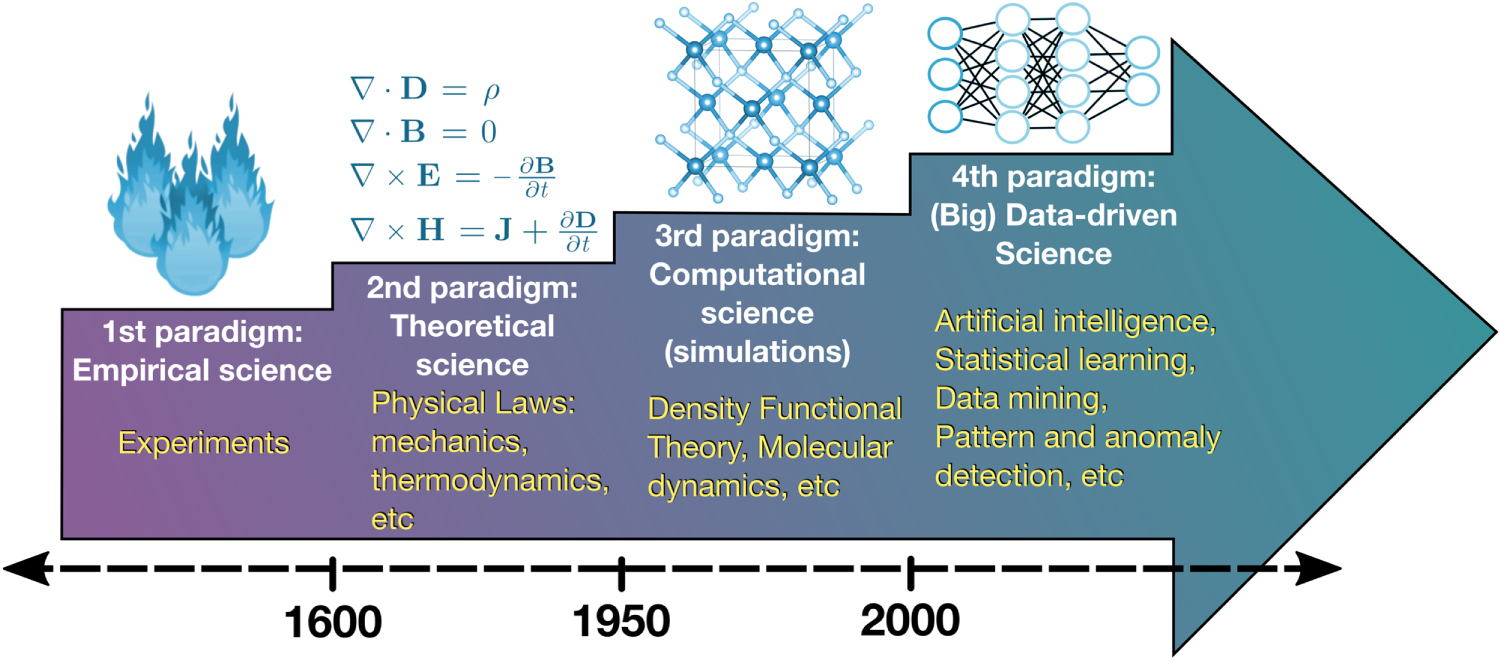
\includegraphics{theory/figures/4th-paradigm-hd.jpg}
  \caption{The four science paradigms: empirical, theoretical, computational, and data-driven. Figure taken from Ref.  \cite{Schleder2019}, which was originally adapted from Ref. \cite{Agrawal2016}.}
  \label{fig:4th-paradigm}
\end{figure}

This chapter aims to provide the neccessary understanding of the new research paradigm in the context of computational materials science and novel materials discovery. Starting from the beginning, we will be looking into information gained by \textit{ab initio} calculations, which means "from first principles". %In particular, it involves a summary of the neccessary theory behind the density functional theory, thus leaving most of the quantum-mechanical world untouched.
Since DFT is not a theory one simply understands, we will begin with an initial discussion of why it is difficult to calculate interactions between particles, followed by a review of key approximations and methods regarding the theory. However, even if density functional theory solves some problems, it also introduces new challenges, which will be thoroughly discussed.

Thereafter, we try to provide a logical sequence into the emergence of high-throughput (HT) methods and tools neccessary to handle the resulting information. Finally, we review a state-of-the-art approach of novel materials discovery enabled by the new paradigm of big data and data science.

\begin{comment}
\section{The single-electron Schrödringer equation}

We will start of investigating the Schrödinger equation with only one electron \cite{Griffiths2017}
\begin{align}
    i\hslash \frac{\partial \Psi}{\partial t} = -\frac{\hslash^2}{2m}\nabla^2 \Psi + V\Psi
    \label{eq:Schrödinger}
\end{align}
for a convenient external potential $V_{ext}(r)$ that is independent of time. We will try to look for solutions for (\autoref{eq:Schrödinger}) by separating the wave function into a space-dependent and time-dependent function
%Most wavefunctions are solutions to (\autoref{eq:Schrödinger}), but if the wavefunction describes a stationary state, the wavefunction has to be an eigenfunction to H for reasons that will become clear shortly.
\begin{align}
  \Psi(r,t) = \psi(r)\phi(t).
  \label{eq:separation}
\end{align}
By inserting ordinary derivatives and dividing each side with equation (\autoref{eq:separation}), our Schrödinger equation (\autoref{eq:Schrödinger}) now reads
\begin{align}
  i\hslash \frac{1}{\phi(t)}\frac{d\phi(t)}{dt} = - \frac{\hslash^2}{2m} \frac{1}{\psi(r)}\nabla^2 \psi + V(r)
\end{align}

Since the potential function $V(r)$ is independent of time, we observe the time and space dependencies of each side and state the fact that both sides has to be constant. Thus, two intriguing equations unveil themselves;
%captivating?
\begin{align}
  i\hslash \frac{1}{\phi(t)}\frac{d\phi(t)}{dt} = E\phi(t)
  \label{eq:time}
\end{align}
and
\begin{align}
  \frac{\hslash^2}{2m} \frac{1}{\psi(r)}\nabla^2 \psi + V(r) = E\psi(r)
  \label{eq:tise}
\end{align}
where the first equation (\autoref{eq:time}) has a general solution $\phi(t) = C \exp (-iEt/\hslash)$ and $C=1$ after normalization, and the second equation (\autoref{eq:tise}) is known as time-independent Schrödinger equation. These two equations are connected through the variable $\varepsilon$.

By utilizing variable separation to get equation (\autoref{eq:separation}), we find that the wavefunction is describing a stationary state with probability density
\begin{align*}
  \lvert \Psi (r,t)\rvert ^2 &= \Psi^*\Psi \\
  &= \Psi^* e^{iEt/\hslash} \Psi e^{-i Et/\hslash} \\
  &= \lvert \Psi (r)\rvert ^2
\end{align*}
that is independent of time. Conveniently, this is also true for every expectation value; they are all constant in time. We can also try to express this in classical terms regarding the Hamiltonian, which in this scenario is defined as
\begin{align}
    \hat{H}(r, p) = \frac{p^2}{2m} + V(r) = -\frac{\hslash^2}{2m}\nabla^2 + V(r)
\end{align}
simplifying equation \autoref{eq:tise} to
\begin{align}
  \hat{H} \psi = E\psi
  \label{eq:tise_nesten}
\end{align}
and we can find the expectation value of the total energy as
\begin{align*}
    \langle H \rangle &= \int \psi^* \hat{H} \psi dr \\
                &= E\int \lvert \Psi \rvert ^2 dr \\
                &= E
\end{align*}
using the fact that expectation values are constant in time for stationary states. Similarly, we can try to estimate the variance of the Hamiltonian,
\begin{align*}
  \sigma_H^2 &= \langle H^2 \rangle - \langle H \rangle ^2 \\
            &= E^2 - E^2 \\
            &= 0
\end{align*}
which appropiately describes that every measurement of the total energy is certain to return the value E.

\subsection{Eigenfunctions}
So far, we have not given an explanation of what a wavefunction is. As a matter of fact, we have actually found an eigenfunction
\begin{align*}
  \psi_\kappa(r,t) = \psi_\kappa e^{-i\varepsilon_\kappa t/\hslash}
\end{align*}
where $\kappa$ denotes the $k$-th eigenfunction and $\varepsilon_\kappa$ is its corresponding energy eigenvalue. The eigenfunctions have distinct energies and have the attribute that they are orthogonal and normalized with respect to
\begin{align*}
  \bra{\psi_\kappa (r,t)} \ket{\psi_{\kappa`} (r,t)} = \delta_{\kappa \kappa'}.
\end{align*}
The state with the lowest energy is called the ground state, and is where it is most likely to find an electron in a single-electron system with no external potential applied.

A general wavefunction can be generated by a summation of eigenfunctions (such as the eigenfunction in the latter case)
\begin{align}
\Psi(r,t) = \sum_\kappa c_\kappa \psi_{\kappa}(r,t),
\end{align}
where $c_\kappa$ is a constant. A general wavefunction does not neccessarily describe stationary states, and consequently does not have distinct energies but is rather represented statistically from the expectation value
\begin{align*}
  E = \sum_{\kappa} \lvert c_\kappa \rvert \varepsilon_\kappa.
\end{align*}
Solving Schrödinger equation for a general wavefunction is rather troublesome. Fortunately, we can use the eigenfunctions instead, transforming equation \autoref{eq:tise_nesten} into time-independent Schrödinger equation for eigenfunctions
\begin{align}
  \hat{H} \psi_{\kappa}(r) = \varepsilon_\kappa \psi_\kappa(r).
\end{align}

The shape of en eigenfunction has normally high spatial symmetri that depends on the symmetri of the potential $V_{ext}(r)$ and the boundary conditions \cite{Persson2020}. The study of how atoms in a crystalline interact with each other is of upmost importance when trying to explain macroscopic consequences.

\end{comment}
\section{Quantum mechanics}
%Before we
%Initially, the method of the calculations can be regarded as a black box where one provides the structure of a material as input, where the black box in return feeds us the outcome in terms of e.g. a different structure. The black box in question is based on a successful theory called density functional theory, which is an approach for predicting physical properties of solid-state systems. %In this and the next section we provide the neccessary knowledge to understand what is happening inside the black box, and the quality of the output.

To fully understand what challenges the density functional theory solves, we will need to introduce a few concepts in quantum mechanics. Quantum mechanics is the fundamental theory which describes nature at microscopic scale. We will only look at the neccessary theory needed to understand the DFT, leaving most of the theory in quantum mechanics untouched.

%Leading up to the density functional theory, we will initially introduce a few concepts required to understand it. Specifically, we will need to utilize the theory of quantum mechanics.

%The significance of this will be crystal clear when we later have to interpret information regarding several thousands solid-state systems, and not a single material. In particular, the quality of the output depends on being consistent.



%Before , we will need to investigate how we can calculate the forces acting inside a crystal. Since these forces are happening on a microscopic scale, we will need to utilize the theory of quantum mechanics.

%However, the fundamental theory remains the same and we will start our venture with the Schrödinger equation.


\subsection{The Schrödinger equation}

In principle, we can describe all physical phenomenas of a system with the wavefunction $\Psi(\boldsymbol{r},t)$ and the Hamiltonian $\hat{H}(\boldsymbol{r},t)$, where $\boldsymbol{r}$ is the spatial position and $t$ is the time. Unfortunately, analytical solutions for the the time-dependent Schrödinger equation,
\begin{align}
    i\hslash \frac{\partial}{\partial t} \Psi(\boldsymbol{r},t) = \hat{H}(\boldsymbol{r},t) \Psi(\boldsymbol{r},t),
    \label{eq:tdse}
\end{align}
are extremely rare. More conveniently, we can generate a general wavefunction by a summation of eigenfunctions,
\begin{align}
  \Psi(\boldsymbol{r},t) = \sum_\kappa c_\kappa \psi_\kappa(\boldsymbol{r},t),
\end{align}
where $c_\kappa$ is a constant and $\psi_\kappa$ is the $\kappa$-th eigenfunction. A general wavefunction does not have distinct energies but is rather represented statistically from the expectation value  %neccessarily describe stationary states, and consequently does not have distrinct energies but is rather represented statistically from the expectation value
\begin{align}
  \left \langle E \right \rangle = \sum_\kappa \lvert c_\kappa \rvert E_\kappa.
\end{align} Solving the Schrödinger equation for a general wavefunction is rather troublesome. However, for a time independent potential, we can use the eigenfunctions and transform \autoref{eq:tdse} into the time-independent Schrödinger equation for eigenfunctions by separation of variables, resulting in
\begin{align}
  \hat{H}\psi_\kappa(\boldsymbol{r}) = E_\kappa \psi_k(\boldsymbol{r}),
\end{align}
where $E_\kappa$ is the eigenvalue of the $\kappa$-th eigenstate $\psi_\kappa(\boldsymbol{r})$. The eigenfunctions have discrete energies, and the state with the lowest energy is called the ground state. They have the attribute that they are orthogonal and normalized with respect to
\begin{align}
  \left \langle \psi_\kappa \left(\boldsymbol{r}\right) \rvert \psi_{\kappa`} \left(\boldsymbol{r} \right) \right \rangle = \delta_{\kappa \kappa'}.
\end{align}
For more information, see Ref. \cite{Griffiths2017}.

\subsection{The many-particle Schrödinger equation}
As we extend the theory to include many-particle systems, we will gradually explain and add the different contributions that make up the many-body Hamiltonian. During this process, we will neglect any external potential applied to the system. \begin{comment}Furthermore, we will apply natural units, that is
\begin{itemize}
  \item Reduced planck constant $\hslash  = 1$.
  \item The magnitute of the charge of the electron $e = 1$.
  \item The electron rest mass $m_e = 1$.
  \item The coloumb force constant $(4\pi\varepsilon_0)^{-1}=1$.
\end{itemize}
\end{comment}

If we place a simple electron with mass $m_e$ in a vacuum, it will be in  possession of kinetic energy. Instead of just one electron, we can place $N_e$ electrons, and they will together have the total kinetic energy
\begin{align}
  T_e = - \sum_{j=1}^{N_e} \frac{\hslash^2\nabla_j}{2m_e}.
\end{align}
All the electrons are negatively charged, causing repulsive Coulomb interactions between each electron, totalling to
\begin{align}
  U_{ee} = \frac{1}{4\pi\varepsilon_0}\sum_{j=1}^{N_e}\sum_{j'<j} \frac{q^2}{\lvert r_j - r_{j'}\rvert},
  \label{eq:electron-electron}
\end{align}
where $\varepsilon$ is the vacuum permittivity. The summation avoids counting each interaction more than once. Simultaneously, we can place $N_n$ nuclei with mass $m_n$ in the same system, accumulating the kinetic energy
\begin{align}
  T_n = - \sum_{a=1}^{N_n} \frac{\hslash^2\nabla_a}{2m_n}.
\end{align}
As in the example with electrons, the nuclei are also experiencing repulsive interactions between every single nucleus, adding up the total interactions as
\begin{align}
  U_{nn} = \frac{1}{4\pi\varepsilon_0}\sum_{a=1}^{N_n}\sum_{a'<a} \frac{q^2 Z_aZ_{a'}}{\lvert R_a - R_{a'}\rvert }.
\end{align}
where $Z_a$ is the atom number of nuclei number $a$. The system now contains $N_e$ electrons and $N_n$ nuclei, thus we need to include the attractive interactions between the them,
\begin{align}
  U_{en} = - \frac{1}{4\pi\varepsilon_0}\sum_{j=1}^{N_e} \sum_{a=1}^{N_n} \frac{q^2Z_a}{\lvert r_j-R_a\rvert}.
\end{align} Together, these equations comprise the time-independent many-particle Hamiltonian
\begin{align}
  \begin{aligned}
    \hat{H} = &- \sum_{j=1}^{N_e} \frac{\hslash^2\nabla_j}{2m_e}
    - \sum_{a=1}^{N_n} \frac{\hslash^2\nabla_a}{2m_n}
    + \frac{1}{4\pi\varepsilon_0} \sum_{j=1}^{N_e}\sum_{j'<j} \frac{q^2}{\lvert r_j - r_{j'}\rvert} \\
    &+\frac{1}{4\pi\varepsilon_0}\sum_{a=1}^{N_n}\sum_{a'<a} \frac{q^2 Z_aZ_{a'}}{\lvert R_a - R_{a'}\rvert } - \frac{1}{4\pi\varepsilon_0}\sum_{j=1}^{N_e} \sum_{a=1}^{N_n} \frac{q^2Z_a}{\lvert r_j-R_a\rvert}.
  \end{aligned}
\end{align} A few problems arise when trying to solve the many-particle Schrödinger equation. Firstly, the amount of atoms in a crystal is very, very massive. As an example, we can numerically try to calculate \autoref{eq:electron-electron} for a $1$ mm$^3$ silicon-crystal that contains $7\cdot 10^{20}$ electrons. For this particular problem, we will pretend to use the current fastest supercomputer Fugaku \cite{Top500} that can calculate $514$ TFlops, and we will assume that we need $2000$ Flops to calculate each term inside the sum \cite{Persson2020}, and we need to calculate it $N_e \cdot N_e/2$ times for the (tiny) crystal.
The entire electron-electron interaction calculation would take $2.46 \cdot 10^{19}$ years to finish for a tiny crystal. Thus, the large amount of particles translates into a challenging numerical problem.

%In one cubic-centimeter of a crystal, there are around $10^{23}$ electrons. This number is roughly the same as the number of stars in the universe, grain of sand on all beaches in the world, or currently $1.41\cdot 10^{19}$ times the amount of Home and Away episodes made since 1988.

Secondly, the many-particle Hamiltonian contains operators that has to be applied to single-particle wavefunctions, and we have no prior knowledge of how $\Psi$ depends on the single-particle wavefunctions $\psi_\kappa$.


\subsection{The Born-Oppenheimer approximation}
The many-particle eigenfunction describes the wavefunction of all the electrons and nuclei and we denote it as $\Psi_{\kappa}^{en}$ for electrons (e) and nuclei (n), respectively. The Born-oppenheimer approximation states that nuclei, of substantially larger mass than electrons, can be treated as fixed point charges. According to this assumption, we can separate the eigenfunction into an electronic part and a nuclear part,
\begin{align}
  \Psi_\kappa^{en}(\boldsymbol{r}, \boldsymbol{R}) \approx \Psi_{\kappa}(\boldsymbol{r}, \boldsymbol{R})\Theta_{\kappa}(\boldsymbol{R}),
\end{align}
where the electronic part is dependent on the nuclei. This is in accordance with the assumption above, since electrons can respond instantaneously to a new position of the much slower nucleus, but this is not true for the opposite scenario. By utilizing this approximation, it can be shown that the equation can be separated into an electronic and a nuclear eigenvalue equation,

\begin{align}
      \left( T_e + U_{ee} + U_{en} \right) \Psi_\kappa (\boldsymbol{r},\boldsymbol{R}) &= E_{\kappa}(\boldsymbol{R})\Psi_\kappa(\boldsymbol{r},\boldsymbol{R})\\
      \left(T_n + U_{nn} + E_\kappa (\boldsymbol{R}) \right) \Theta_\kappa(\boldsymbol{R}) &= E_{\kappa}^{en}(\boldsymbol{R})\Theta_\kappa(\boldsymbol{r},\boldsymbol{R}),
\end{align}
where the two equations are coupled by the electronic energy eigenvalue $E_{\kappa}(\boldsymbol{R})$. Since we can consider the nuclei as point charges, it is common to set the kinetic energy of the nuclei, $T_n$, to zero. Thus, the left side of the nuclear eigenvalue equation is shortened down to the terms $\left(U_{nn} + E_\kappa (\boldsymbol{R}) \right)$, which is denoted as the potential energy surface (PES), $E_p(\boldsymbol{R})$.
%From here, one can obtain the electronic and nuclear eigenfunction, with the derivation shown in Appendix \ref{appendix:Born-Oppenheimer}.


\subsection{The Hartree and Hartree-Fock approximations}
\begin{comment}
As we venture along from a one-electron system to a two-electron systen, we encounter a new wavefunction and Hamiltonian that needs to describe two particles, making the two-electron Schrödinger equation read

\begin{align}
  \Big( -\frac{\hslash^2 \nabla_1^2}{2m_e} - \frac{\hslash^2\nabla_2^2}{2m_e}+ \frac{q^2}{\lvert r_1-r_2  \rvert} + V_{ext}(r) \Big) \Psi_\kappa (r_1, r_2) = E_{\kappa} \Psi_\kappa (r_1, r_2),
\end{align}
where the two first terms are the kinetic energies of the electrons, while the third term is a potential that describes the repulsive Coloumb interaction between the two electrons. The last term is the external potential, well known from the earlier scenario with only one electron.
\end{comment}
The next question in line is to find a wavefunction $\Psi(\boldsymbol{r},\boldsymbol{R})$ that describes all of the electrons in the system. The Hartree \cite{Persson2020, DavidSholl2009} approximation to this is to assume that electrons can be described independently, suggesting the \textit{ansatz} for a two-electron wavefunction
\begin{align}
  \Psi_\kappa(\boldsymbol{r}_1,\boldsymbol{r}_2) = A \cdot \psi_1(\boldsymbol{r}_1) \psi_2(\boldsymbol{r}_2),
\end{align}
where $A$ is a normalization constant. This approximation simplifies the many-particle Shrödinger equation a lot, but comes with the downside that the particles are distinguishable and do not obey the Pauli exclusion principle for fermions.

The Hartree-Fock approach, however, overcame this challenge and presented an anti-symmetric wavefunction that made the electrons indistinguishable \cite{Griffiths2017}:
\begin{align}
  \Psi_\kappa(\boldsymbol{r}_1,\boldsymbol{r}_2) = \frac{1}{\sqrt{2}}\Big( \psi_1(\boldsymbol{r}_1) \psi_2(\boldsymbol{r}_2)  - {\psi_1(\boldsymbol{r}_2)\psi_2(\boldsymbol{r}_1)}\Big).
\end{align}
%For systems containing more than one particles, the factor $1/\sqrt{2}$ becomes the Slater determinant and is used to normalize the wave function.

\subsection{The variational principle}
So far, we have tried to make the time-independent Schrödinger equation easier with the use of an \textit{ansatz}, but we do not neccessarily have an adequate guess for the eigenfunctions and the ansatz can only give a rough estimate in most scenarios. Another approach, namely the \textit{variational principle}, states that the energy of any trial wavefunction is always an upper bound to the exact ground state energy by definition $E_0$,
\begin{align}
  E_0 = \bra{\psi_0 } H \ket{\psi_0} \leq \bra{\psi}H\ket{\psi} = E
  \label{eq:variational}
\end{align} This enables a minimization of energy in terms of wavefunction parameters. A more thorough walk-through of the variational principle is included in Appendix \ref{appendix:variational-principle}.

\section{The density functional theory}

Hitherto we have tried to solve the Schrödinger equation to get a ground state wave function, and from there we can obtain ground state properties. One fundamental problem that exists when trying to solve the many-electron Schrödinger equation is that the wavefunction is a complicated function that depends on $3N_e$ variables\footnote{not including spin}.

Hohenberg and Kohn \cite{Hohenberg1964} showed in 1964 that the ground-state density $n_0(r) = \lvert \Psi_0 (r)\rvert$ determines a general external potential, which includes $U_{en}$, up to an additive constant, and thus also the Hamiltonian \cite{Toulouse2019}. From another point of view, the theory states that all physical ground-state properties of the many-electron system are unique functionals of the density \cite{Persson2020}. A consequence of this is that the number of variables is reduced from $3N_e$ to $3$, significantly reducing the computational efforts.

However, the scheme is not without limitations, as the density functional theory (DFT) can only be used to find all the ground-state physical properties if the exact functional of the electron density is known. And $57$ years after Hohenberg and Kohn published their paper, the exact functional still remains unknown.

We will start this chapter with a brief mention of the Hohenberg-Kohn theorems and its implications, before we delve further into the Kohn-Sham equation.

\subsection{The Hohenberg-Kohn theorems}

\begin{theorem}
  For any system of interacting particles in an external potential $V_{ext}$, the density is uniquely determined.
\end{theorem}

The theorem can be proved by utilising the variational principle for two different external potentials with the same ground state density.
The proof is included in Appendix \ref{appendix:theorem1}.

\begin{theorem}
  There exists a variational principle for the energy density functional such that, if $n$ is not the electron density of the ground state, then $E\left[ n_0 \right] < E\left[ n \right]$.
\end{theorem}

From theorem 1, we know that the external potential is uniquely determined by the density, which in turn uniquely determines the ground state wavefunction. Therefore, all other observables of the system are uniquely determined and we can express the energy as function of the density,
\begin{align}
  E[n] = \overbrace{T[n] + U_{ee}[n]}^{F[n]} + U_{en}[n],
  \label{eq:densityfunctional}
\end{align}
where $F[n]$ is an universel functional known as the Hohenberg-Kohn functional. The proof for theorem 2 is found in Appendix \ref{appendix:theorem2}.

\subsection{The Kohn-Sham equation}
So far, we have tried to make the challenging Schrödinger equation less challenging by simplifying it. The last attempt of simplifying it involved the Hohenberg-Kohn's theorems where the theory states that the total ground-state energy can, in principle, be determined exactly once we have found the ground-state density.

In 1965, Kohn and Sham \cite{Kohn1965} reformulated the Hohenberg-Kohn theorems by generating the exact ground-state density $n_0(r)$ using a Hartree-like total wavefunction
\begin{align}
    \Psi(\boldsymbol{r}_1,\boldsymbol{r}_2,..,\boldsymbol{r}_{N_e}) = \psi_1^{KS}(\boldsymbol{r}_2)\psi_2^{KS}(\boldsymbol{r}_2)...\psi_{N_e}^{KS}(\boldsymbol{r}_{N_e}),
\end{align}
where $\psi_j^{KS}(r_j)$ are some auxiliary independent single-particle wavefunctions. However, the Kohn-Sham wavefunctions cannot be the correct single-particle wavefunctions since our ansatz implies an exact density
\begin{align}
  n(\boldsymbol{r}) = \sum_{j=1}^{N_e}\lvert \psi_j^{KS}(\boldsymbol{r})\rvert^2.
\end{align}
Recalling that equation \autoref{eq:densityfunctional} describes the total energy as a functional of the density,
\begin{align}
  E[n] = T[n] + U_{ee}[n] + U_{en}[n],
\end{align}
we try to modify it to include the kinetic energy $T_s[n]$ and the interaction energy $U_s[n]$ of the auxiliary wavefunction, with the denotation $s$ for single-particle wavefunctions.
\begin{align*}
  E[n] &= T[n] + U_{ee}[n] + U_{en}[n] + \left( T_s[n] - T_s[n] \right) + \left( U_s[n] - U_s[n] \right) \\
  &= T_s[n] + U_{s}[n] + U_{en}[n] + \underbrace{\left(T[n] - T_s[n] \right) + \left( U_{ee}[n] - U_s[n] \right)}_{E_{xc}[n]}
\end{align*}
Here we have our first encounter with the \textit{exchange-correlation energy}
\begin{align}
  E_{xc}[n] = \Delta T + \Delta U = \left(T[n] - T_s[n] \right) + \left( U_{ee}[n] - U_s[n] \right),
\end{align}
which contains the complex many-electron interaction. For non-interacting systems, $E_{xc}[n]$ is conveniently zero, but in interacting systems it most likely is a complex expression. However, one can consider it as our mission to find good approximations to this term, as the better approximations, the closer we get to the exact expression.

The exact total energy functional can now be expressed as
\begin{align}
  \begin{aligned}
  E[n]
  &= \overbrace{\sum_j \int \psi_j^{KS*} \frac{-\hslash^2\nabla^2}{2m} \psi_j^{KS}d\boldsymbol{r}}^{T_s[n]} + \overbrace{\frac{1}{2}\frac{1}{4\pi\varepsilon_0}\int \int q^2\frac{n(\boldsymbol{r})n(\boldsymbol{r}')}{\lvert \boldsymbol{r}-\boldsymbol{r}'\rvert} d\boldsymbol{r}d\boldsymbol{r}'}^{U_s[n]}
  \\ &+ \underbrace{\int V_{en}(\boldsymbol{r})n(\boldsymbol{r})d\boldsymbol{r}}_{U_{en}[n]} + \underbrace{\left(T[n] - T_s[n] \right) + \left( U_{ee}[n] - U_s[n] \right)}_{E_{xc[n]}},
  \end{aligned}
\end{align}
given that the exchange-correlation functional is described correctly. By utilizing the variational principle, we can now formulate a set of Kohn-Sham single-electron equations,
\begin{align}
  \left\{ -\frac{\hslash^2}{2m_e}\nabla^2_s + V_H(\boldsymbol{r}) + V_{en}(\boldsymbol{r}) + V_{xc}(\boldsymbol{r}) \right\} \psi_s^{KS}(\boldsymbol{r}) = \epsilon_s^{KS} \psi_s^{KS}(\boldsymbol{r}),
  \label{eq:singleKS}
\end{align}
where $V_{xc}(\boldsymbol{r})=\partial E_{xc}[n]/\partial n(\boldsymbol{r})$ and $V_{H}(\boldsymbol{r})=\frac{1}{4\pi\varepsilon_0}\int q^2 \frac{n(\boldsymbol{r'})}{\lvert \boldsymbol{r} - \boldsymbol{r}'\rvert} d\boldsymbol{r}'$ is the Hartree potential describing the electron-electron interaction.
It is worth to notice that $V_H(\boldsymbol{r})$ allows an electron to interact with itself, resulting in a self-interaction contribution, however this can be taken care of in $V_{xc}$.

Finally, we can define the total energy of the system according to Kohn-Sham theory as
\begin{align}
  E[n] = \sum_{j}\epsilon_j^{KS}-\frac{1}{2}\frac{1}{4\pi\varepsilon_0}\int \int q^2 \frac{n(\boldsymbol{r})n(\boldsymbol{r}')}{\lvert \boldsymbol{r} - \boldsymbol{r}' \rvert} d\boldsymbol{r}d\boldsymbol{r}' + E_{xc}[n] - \int V_{xc}(\boldsymbol{r})n(\boldsymbol{r})d\boldsymbol{r}.
\end{align}
If $V_{xc}$ is exact, and $E[n]$ gives the true total energy, we still do not know if the energy eigenvalues $\epsilon_s^{KS}$ are the true single-electron eigenvalues. However, there exists one exception, which is that the highest occupied eigenvalue of a finite system has to be exact if the density is exact.

The only task that is left for us now is to find the exact expression for $E_{xc}[n]$ as a functional of the density $n(r)$. With that expression, we would be able to calculate the total energies of any material. %, and most likely solve a few of the biggest puzzles in the history of humankind.
Unfortunately, the exchange-correlation potential is unknown for most systems.

It is possible to solve the Kohn-Sham equations by applying a self-consistent field method. This is a computational scheme, and for further details one can consult the Appendix \ref{appendix:self-consistent}.

%In this approximation we have used Hartree energy where the self-interaction correction is neglected, raising less accurate results. It is possible to use other approximations for $T_s[n]$ and $U_s[n]$ than Hartree wavefunctions, and good approximations will result in a low $E_{xc}[n]$ because $T_s[n]$ and $U_s[n]$ will get closer and closer to the true values.


%The next step in finding the KS-equation is to utilize the variational principle in the purpose of finding the ground-state energy. First one minimises the total energy with respect to each of the wavefunctions with the constraint that the wavefunctions should be orthonormalized;
%\begin{align*}
%  \frac{\partial }{\partial \psi_j^{*} (\boldsymbol{r})}E[n] &= \sum_{i,j}\lambda_{ij}\int \psi_i^{s*}(\boldsymbol{r}_i)\psi_j^{s}(\boldsymbol{r}_j)d\boldsymbol{r}d\boldsymbol{r}_j\\
%  \frac{\partial }{\partial \psi_j^{*} (\boldsymbol{r})}E[n] &= \lambda_j\psi_j^s (\boldsymbol{r}_j)
%\end{align*}

\subsection{The exchange-correlation energy}


There is one scenario for which we can derive the exact expression of the exchange-correlation functional, namely the \textit{homogeneous electron gas} (HEG). However, this has a natural cause, since by definition $n(\boldsymbol{r})$ is constant for this situation. Given that it is the variations of electron density that are the foundation of material properties, the usefulness of HEG is limited. The \textit{local density approximation} (LDA) is an approximation based on this approach, where the local density is the only variable used to define the exchange-correlation functional. Specifically, we can set the exchange-correlation potential at each position to be the known exchange-correlation potential from homogeneous electron gas at the electron density observed at that position \cite{Kohn1965}:
\begin{align}
  V_{xc}(\boldsymbol{r}) = V_{xc}^{\text{electron gas }}\left[n(\boldsymbol{r})\right].
\end{align}
This is the simplest and most known approximation to the exchange-correlation functional, and accordingly it has a few drawbacks. One of them is the incomplete cancellation of the self-interaction term, which leads to a repulsion that may cause artifical repulsion between electrons, and hence increased electron delocalization \cite{Allen2014}. In addition, LDA has proven challenging  to use when studying atoms and molecules because of their rapidly varying electron densities, however, the LDA is seen as succesful for bulk materials because of the slowly varying electron density \cite{DavidSholl2009}. Considering the relatively low computational cost and relatively high accuracy, the LDA overall makes a good model for estimation of the exchange-correlation functional for bulk-materials.

In the light of the merits of the LDA, an extensive search for new approximations was launched. The \textit{generalized gradient approximation} (GGA) is an extension of the LDA, which includes the gradient of the density
\begin{align}
  V_{xc}^{GGA}(\boldsymbol{r}) = V_{xc}\left[ n(\boldsymbol{r}), \nabla n (\boldsymbol{r})\right].
\end{align}
The GGA is a good approximation for the cases where the electron density varies slowly, but faces difficulties in many materials with rapidly varying gradients in the density, causing the GGA to fail. Thus, the annotation \textit{generalized} in GGA is set to include the different approaches to deal with this challenge. Two of the most commonly implemented GGA functionals are the non-empirical approaches Perdew-Wang 91 (PW91) \cite{Perdew1992} and Perdew-Burke-Ernzerhof (PBE) \cite{Perdew1996}.

Both LDA and GGA are commonly known to severely underestimate the band gaps of semiconductor materials, in addition to incorrectly predicting charge localizations originating from narrow bands or associated with local lattice distortions around defects \cite{Freysoldt2014}. The latter limitation is thought to be due to self-interaction in the Hartree potential in \autoref{eq:singleKS}.
\begin{comment}
To improve the accuracy of excited state properties estimations, other methods have been developed. Tran and Blaha (TB) \cite{Tran2009} adapted the exchange potential suggested by Becke-Roussel (BR) \cite{Becke2006} that leads to band gaps close to experimental values while still using a cheap semilocal method \cite{Koller2011}. The modified TB-mBJ version introduces a parameter relative to the BJ version,
\begin{align}
    V_{xc}^{TB-mBJ}(\boldsymbol{r}) =  c\cdot V_{xc}^{BR}(\boldsymbol{r}) + (3c-2) \frac{1}{\pi} \sqrt{\frac{5}{6}} \sqrt{\frac{t(\boldsymbol{r})}{\rho(\boldsymbol{r})}},
\end{align}
where $\rho$ is the electron density, $t$ is the kinetic-energy density, $V_{xc}^{BR}$ is the Becke-Roussel exchange potential and $c$ is the parameter that changes weights of the BJ potential and is fit to experimental data.
\end{comment}
Hybrid functionals intermix exact Hartree-Fock exchange with exchange and correlation from functionals based on the LDA or GGA. Hartree-Fock theory completely ignores correlation effects, but accounts for self-interaction and treats exchange as exact. Since LDA/GGA and Hartree-Fock supplement each other, they can be used as a combination for hybrid-functionals resulting in some cancellation of the self-interaction error. Becke \cite{Becke1993} introduced a $50\%$ Hartree-Fock exact exchange and
$50\%$ LDA energy functional, while Perdew \textit{et al.} \cite{Perdew1996a} altered it to $25\%-75\%$ and favoring PBE-GGA instead of LDA.

The inclusion of Hartree Fock exchange improves the description of localized states, but requires significantly more computational power for large systems. Another method called the \textit{GW} approximation includes screening of the exchange interaction \cite{Aryasetiawan1998}, but has a computational price that does not neccessarily defend its use. Thus, the real challenge is to reduce the computational effort while still producing satisfactory results. Heyd \textit{et al.} \cite{Heyd2003} suggested to separate the non-local Hartree-Fock exchange into a short- and long-range portion, incorporating the exact exchange in the short-range contribution. The separation is controlled by an adjustable parameter $\omega$, which was empirically optimised for molecules to $\omega = 0.15$ and solids to $\omega = 0.11$ and are known as the HSE03 and HSE06 (Heyd-Scuseria-Ernzerhof), respectively \cite{Krukau2006}. The functionals are expressed as
\begin{align}
  E_{xc}^{HSE} = aE_{x}^{\text{HF,SR}}(\omega) + (1-a)E_x^{\text{PBE,SR}}(\omega) + E_x^{\text{PBE,LR}}(\omega) + E_c^{\text{PBE}}
\end{align}
where $a=1/4$ is the Hartree-Fock mixing constant and the abbreviations SR and LR stands for short range and long range, respectively.

Hence, hybrid-functionals are \textit{semi-empirical} functionals that rely on experimental data for accurate results. They give accurate results for several properties, such as energetics, bandgaps and lattice parameters, and can fine-tune parameters fitted to experimental data for even higher accuracy.

Furthermore, the computational effort required for the hybrid-functionals are significantly larger than for non-empirical functionals such as LDA or GGA. Krukau \textit{et al.} \cite{Krukau2006} reported a substantial increase in computational cost when reducing the parameter $\omega$ from $0.20$ to $0.2$ for 25 solids, and going lower than $0.11$ demanded too much  to actually defend its use.
\begin{comment}
Unfortunately, an area where both GGA and hybrid functionals are reportedly inadequate is in calculating the dispersion interactions \cite{Klimes2009}. Many implementations have been developed to deal with this vulnerability, with one of them being the non-local van der Waals density functional (vdW-DF) \cite{Dion2004}
\begin{align}
  E_{xc} = E_{x}^{GGA} + E_{c}^{\text{LDA}} + E_{c}^{nl},
\end{align}
where $E_{x}^{GGA}$ is GGA exchange energy \cite{Klimes2009}.
\end{comment}
\subsection{Limitations of the DFT}

If we had known the exact exchange-correlation functional, the density functional theory would yield the exact total energy. Alas, that is not the case and we are bound to use approximations in forms of functionals. What is common for all approximations is that they are specifically designed to solve one given optimization in DFT, therefore it is not neccessarily one functional that is considered superior in all fields of interest. One could consider that the hybrid functionals due to a high accuracy overall should be dominant, but that is only if one has the computational capacity required. The accuracy of calculations depends on which functional is used, and normally a higher accuracy means the use of a more complex and computationally demanding functional.

Additionally, one can almost never be certain if a DFT-calculation has found a local or global minima. There is an unknown associated uncertainty of every calculation, which has to be taken into consideration. Nonetheless, density functional theory is considered a very successful approach and Walter Kohn was awarded the Nobel Price in chemistry in 1998 for his development of the density-functional theory \cite{Freitas1999}. It has matured into the undisputed choice of method for electronic structure calculations \cite{Schleder2019}. It is especially regarded as successful in contexts where DFT can make important contributions to scientific questions where it would be essentially impossible to determine through experiments \cite{DavidSholl2009}. %One can only hope that the future will be as bright as the past, and that this successful theory provides incentives for further growth in the next generation.

\section{High-throughput information storage}


Fuelled by the widespread application of DFT in material science, we observe an increase of computational capacity due to advances in simulation methods, computational science and technologies \cite{Schleder2019}. The time required for calculations has been reduced substantially, and enables more time to be spent on simulation setup and analysis. Ultimately, this has led to a new type of workflow called high-throughput (HT) \cite{Yang2017}, where one can automate input creation and perform several (up to millions) simulations in parallel instead of performing many manually-prepared simulations. The HT engines are required to be fast and accurate, otherwise the purpose of its existence is lost. We will in this thesis mainly focus on high throughput in the context of first principles DFT calculations.

Normally, the implementation of HT-DFT methods is done in three steps. In the first step we perform thermodynamic or electronic structure calculations for a large number of materials. For the second step, we store the information gathered in a systematic database, normally known as a material repository. For the third and final step, we characterize and select novel materials or analyse and extract new physical insight \cite{Schleder2019}. In general, the two first steps are performed on high-performance computers (HPC), and are defining for the third step due to the vast amount of interesting properties of materials. Importantly, one needs to consider the ultimate goal in step three initially before deciding upon materials and properties to calculate.

One of the largest government funded projects is the $2011$ launched Material Genome Initiative (MGI) \cite{Warren2018} which seeks to accelerate the discovery, design, development and deployment of novel materials through the creation of a materials innovation infrastructure.
As a result, we have seen an intensive implementation of material repositories that fascilitate sharing and distribution of step $1$ and $2$, with the ultimate goal of storing calculated properties of all feasible structures of materials \cite{Schuett2020}.
Examples include AFLOW \cite{Curtarolo2012, Curtarolo2012a, Calderon2015}, Materials Project \cite{Jain2013, Jain2018} , OQMD \cite{Saal2013, Kirklin2015} and JARVIS-DFT \cite{Choudhary2020}.
On the other hand, we find a less diverse selection of experimental databases, with perhaps the most known being the Inorganic Crystal Structure Database (ICSD) \cite{Allen1987}.

In this section, we describe a few of the most widely known high-throughput databases, codes and tools, with an emphasis of what the particular speciality of each database is.

\subsection{Materials project}

Materials project \cite{Jain2013, Jain2018} is an open source project that is based on the Vienna Ab Initio Software Package (VASP) \cite{Kresse1996}, and offers a variety of properties of over one hundred thousand inorganic crystalline materials. It is known as the initiator of materials genomics and has as its mission to accelerate the discovery of new technological materials, with an emphasis on batteries and electrodes, through advanced scientific computing and innovative design.

 %Some features, eg. density of state (dos), bandstructure, Pourbaix diagram etc., are characterized by using the module pymatgen.

Every compound has an initial relaxation of cell and lattice parameters performed using a $1000$ / (number of atoms in cell) k-point mesh to ensure that all properties calculated are representative of the idealized unit cell for each respective crystal structure \cite{Ferrenti2020}. The functional GGA is used to calculate band structures, while for transition metals, a $+U$ corrections is applied to correct for correlation effects in d- and f-orbital systems that are not addressed by GGA calculations \cite{Wang2006}.

To adress that many compounds are not thermodynamically stable, which means that they do not appear on any phase stability diagrams \cite{Sun2016}, an additional metric has been added. This metric is based on a convex hull analysis, where compounds on the convex hull are stable, while compounds above the hull in terms of energy are metastable \cite{Jain2018}. This is denoted as energy above hull (E Above Hull), where a value of zero is defined as the most stable phase at a given composition, while larger positive values indicate increased instability.

%The thermodynamic stability for each phase with respect to decomposition, is also calculated.
Each material contains multiple computations for different purposes, resulting in different 'tasks'. The reason behind this is that each computation has a purpose, such as to calculate the band structure or energy. Therefore, it is possible to receive several tasks for one material.

\subsection{AFLOW}

The AFLOW\cite{Curtarolo2012, Curtarolo2012a, Calderon2015} repository is an automatic software framework for the calculations of a wide range of inorganic material properties. They utilise the GGA-PBE functional within VASP with projector-augmented wavefunction (PAW) potentials to relax twice and optimize the ICSD-sourced structure. They are using a $3000$ to $6000$ / (number of atoms in cell) $k$-point mesh, indicating a more computationally expensive calculation compared to the Materials Project \cite{Ferrenti2020}. Next, the band structure is calculated with an even higher $k$-point density, in addition to the $+U$ correction term for most occupied d- and f-orbital systems \cite{Setyawan2010}. Furthermore, they apply a standard fit gathered from a study of DFT-computed versus experimentally measured band gap widths to the initial calculated value, obtaining a fitted band gap \cite{Setyawan2011}.

\subsection{Open Quantum Materials Database}

The Open Quantum Materials Database (OQDM) \cite{Saal2013, Kirklin2015} is a free and available database of DFT-calculations. It contains thermodynamic and structural properties of more than $600.000$ materials, including all unique compounds in the Inorganic Crystal Structure Database (ICSD) that consists of less than $34$ atoms \cite{Ferrenti2020}.

The DFT calculations are performed with the VASP software whereas the electron exchange and correlation are described with the GGA-PBE, while using the PAW potentials. They relax a structure using $4000-8000$ / (number of atoms in cell) $k$-point mesh, indicating an even more computationally expensive calculation than AFLOW \cite{Ferrenti2020}. Several element-specific settings are included such as using the $+U$ extension for various transition metals, lanthanides and actinides. In addition, any calculation containing 3d or actinide elements are spin-polarized with a ferromagnetic alignment of spins to capture possible magnetism. However, the authors note that this approach does not capture complex magnetic properties such as antiferromagnetism, which has been found to result in substantial errors for the formation energy \cite{Stevanovic2012}.

\subsection{JARVIS}

Joint Automated Repository for Various Integrated Simulations (JARVIS) - DFT \cite{Choudhary2020} is an open database based on the VASP \cite{Kresse1996} software to perform a variety of material property calculations. It consists of roughly $40.000$ 3D and $1.000$ 2D materials using the vdW-DF-OptB88 van der Waals (vdW) functional, which was originally designed to improve the approximation of properties of two-dimensional van der Waals materials, but was also shown to be effective for bulk materials \cite{Thonhauser2007, Klimes2011}. The functional has yielded accurate predictions for lattice-parameters and energetics for both vdW and non-vdW bonded materials  \cite{Choudhary2018}.

Structures included in the data set are originally taken from the Materials Project, and then re-optimized using the OPT-functional. Finally, the combination of the OPT and modified Becke-Johnson (mBJ) functionals are used to obtain a representative band gap of each structure \cite{Choudhary2018a}. %, since both have shown unprecedented accuracy in the calculation of band gap compared to any other DFT-based calculation methods \cite{Choudhary2018a}.
The JARVIS-DFT database is part of a bigger platform that includes JARVIS-FF, which is the evaluation of classical forcefield with respect to DFT-data, and JARVIS-ML, which is a repository of machine learning model parameters and descriptors.
%which consists of 25 machine learning descriptors to predict properties of materials.
In addition, JARVIS-DFT also includes a data set of 1D-nanowire and 0D-molecular materials, which is not yet publically distributed.

\section{Materials informatics}

Despite a computationally demanding step $1$ and a sophisticated database architecture defined in step $2$, the third step remains more important in discovery of novel materials. In the third step, we apply constraints to the database in order to filter or select the best candidates according to the desired attributes \cite{Schleder2019}, and is referred to as data \textit{mining} and data \textit{screening}. To achieve the most insight, we normally apply the constraints in a sequential manner to identify any potential underlying trend. The materials that satisfy the first constraint move on to the next round, while the rest are eliminated from further consideration. The constraints can be applied either by the understanding of properties, human intuition or through a close interaction with a machine learning (ML) algorithm, where the latter will be extensively studied in the next chapter.

\begin{figure}[ht!]
  \centering
  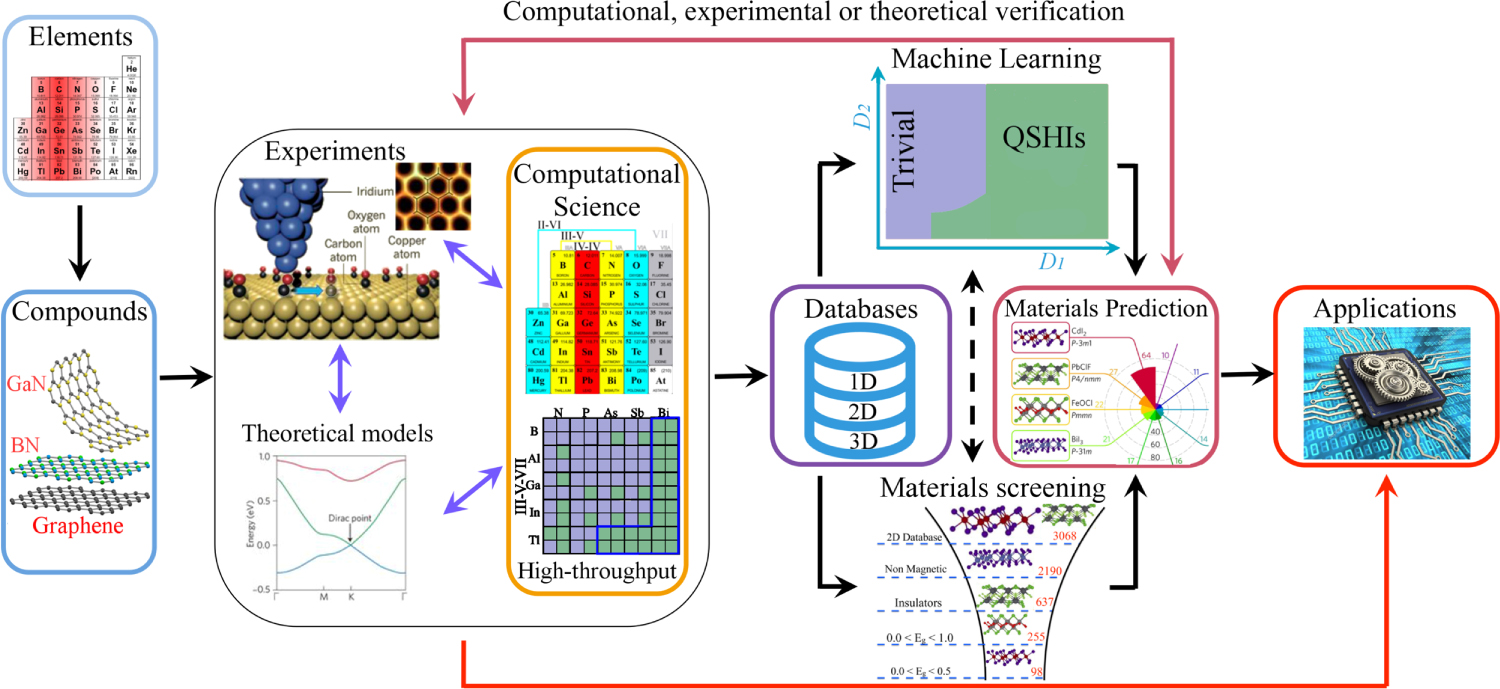
\includegraphics{theory/figures/ht-workflow.jpg}
  \caption{Schematic representation of the workflow of novel materials discovery.  Figure taken from Ref. \cite{Schleder2019}, which was originally adapted from Refs. \cite{Mounet2018, Acosta2018, Polini2013}.}
  \label{fig:ht-workflow}
\end{figure}

\noindent Together, the three steps resemble \autoref{fig:ht-workflow}. From building compounds based on elements, calculating theoretical, computational and experimental properties, storing the information in databases and applying material screening and machine learning, to finally receiving a material prediction. If the material prediction is verified iteratively by many independent sources, the time to market for new technologies based on a new material takes approximately $20$ years \cite{Eagar1995, Schleder2019}.

Importantly, the data driven paradigm enables a new approach for novel material discovery. The traditional approach, namely the \textit{direct approach}, relies on the calculation of properties given the structure and composition of a material, such that the search for eligible candidates exhibiting the target property is performed tediously case by case. In other words, what is the property of a given material. However, the \textit{inverse approach} is of integral importance in this work: given a desired property, what material can present it \cite{Schleder2019}?

The application of machine learning and data-driven techniques to material science has developed into a new field named \textit{materials informatics} \cite{Rajan2005}. Alex Szalay, director of the US National Virtual Observatory project, described informatics for astronomy in $2003$ as the following:
\begin{quote}
   ``Science was originally empirical, like Leonardo making wonderful drawings of nature. Next came the theorists who tried to write down equations that explained observed behaviors, like Kepler or Einstein. Then, when we got to complex enough systems like the clustering of a million galaxies, there came the computer simulations – the computational branch of science. Now, we are getting into the data exploration part of science, which is kind of a little bit of them all'' Alex Szalay \cite{Szalay2003}
\end{quote}
\noindent The formulation is true also for materials informatics, where the scope is to discover relations between known standard features and material properties through a combination of \emph{a bit of everything}.

\subsection{Materials informatics software packages}

In practice, several software packages exists for the purpose of generating, describing, visualizing, calculating or predicting properties of materials.

The Atomic Simulation Environment (ASE) is an environment in the Python programming language that includes several tools and modules for setting up, modifying and evaluate atomistic simulations \cite{Larsen2017}. It is in particular used together with the Computational Materials Repository (CMR) \cite{Landis2012}.

Another commonly used module is the Python Materials Genomics (pymatgen) \cite{Ong2013}. This is a well-documented open module with both introductory and advanced use case examples written in Jupyter Notebook for easy reproducibility, and is integrated with the Materials Project. %RESTful API.

An increasingly popular library is Matminer \cite{Ward2018}, which is an open-source toolkit for material analysis written in Python. Matminer is powered by a group known as \textit{Hacking Materials Research Group}\footnote{Project's Github site: https://github.com/hackingmaterials.}. Matminer provides modules to extract data information from a wide variety of databases. Additionally, they provide the tools to construct possibly thousands of features from calculations based on a materials composition, structure and DFT-calculations, and have modules for visualization and automatic machine learning.

AFLOW-ML \cite{Isayev2017} is an API that uses machine learning to predict thermomechanical and electronic properties based on the chemical composition and atomic structure alone, which they denote as \textit{fragment descriptors}. They start with applying a classification model to predict if a compound is either a metal or an insulator, where the latter is confirmed with an additional regression model to predict the band gap width. To be able to predict properties on an independent data set, they utilise a fivefold cross validation process for each model. They report a $93$\% prediction success rate of their initial binary classification model, whereas the majority of the wrongful predictions are narrow-gap semiconductors. It has been found that $93$\% of the machine-learning-derived values are within $25$\% of the DFT $+U$-calculated band gap width \cite{Ferrenti2020}.

%The authors does not compare their predicted band gap to experimental values, but it is found that $93$\% of the machine-learning-derived values are within $25$\% of the DFT $+U$-calculated band gap width \cite{Ferrenti2020}.

\subsection{Associated challenges with materials informatics}

%Despite the new and promising methods recently

Despite the promising methods recently developed for novel materials discovery, there are considerable challenges that need to be adressed.

The data generated by HT-DFT are estimates of varying degree depending on functional applied. In perspective of this work, we emphasis the underestimation of predicted band gaps. In particular, we find that the (arguably) most popular materials science database Materials Project estimates band gaps with the GGA functional (+U for transition metals). If we were to use their data, it is important to validate its quality, such that we can draw conclusions with the correct information at hand.

Furthermore, out of the (so far) $118$ discovered elements, there are potentially millions of combinations that constitute distinct materials. Only a small fraction of these materials have their basic properties determined \cite{Springer2017}. If we were to involve all combinations of surfaces, nanostructures and inorganic materials, the complexity would increase substantially. This has two consequences. Firstly, due to the small number of determined properties, we are bound to continue with estimates for probably a long time. Perhaps more optimistic is the second consequence, since it is reasonable to believe that materials with promising properties are still to be discovered in almost every field \cite{Pedregosa2012}.

We are in the beginning of a new era, with new technological advances happening every day. By acknowledging and overcoming the challenges, we believe the future is looking bright for material informatics.

        
\chapter{The density functional theory}

Hitherto we have tried to solve the Schrödinger equation to get a ground state wave function, and from there we can obtain ground state properties, such as the ground state total energy. One fundamental problem that exists when trying to solve the many-electron Schrödinger equation is that the wavefunction is a complicated function that depends on $3N_e$ variables\footnote{not including spin}.

Hohenberg and Kohn \cite{Hohenberg1964} showed in 1964 that the ground-state density $n_0(r) = \lvert \Psi_0 (r)\rvert$ determines a general external potential, which includes $U_{en}$, up to an additive constant, and thus also the Hamiltonian \cite{Toulouse2019}. From another point of view, the theory states that all physical ground-state properties of the many-electron system are unique functionals of the density \cite{Persson2020}. A consequence of this is that the number of variables is reduced from $3N_e$ to $3$, significantly reducing the computational efforts.

However, the scheme is not without limitations, as the density functional theory (DFT) can only be used to find all the ground-state physical properties if the exact functional of the electron density is known. And $56$ years after Hohenberg and Kohn published their paper, the exact functional still remains unknown.

We will start this chapter with a discussion of the Hohenberg-Kohn theorems, before we delve further into the Kohn-Sham equation.

\section{The Hohenberg-Kohn theorems}

\begin{theorem}
  For any system of interacting particles in an external potential $V_{ext}$, the density is uniquely determined.
\end{theorem}
\begin{proof}
  Assume that two external potentials $V_{ext}^{(1)}$ and $V_{ext}^{(2)}$, that differ by more than a constant, have the same ground state density $n_0(r)$. The two different potentials correspond to distinct Hamiltonians $\hat{H}_{ext}^{(1)}$ and $\hat{H}_{ext}^{(2)}$, which again give rise to distinct wavefunctions $\Psi_{ext}^{(1)}$ and $\Psi_{ext}^{(2)}$. Utilizing the variational principle, we find that no wavefunction can give an energy that is less than the energy of $\Psi_{ext}^{(1)}$ for $\hat{H}_{ext}^{(1)}$, that is
  \begin{align}
    E^{(1)} = \bra{\Psi^{(1)}}\hat{H}^{(1)}\ket{\Psi^{(1)}} &< \bra{\Psi^{(2)}}\hat{H}^{(1)}\ket{\Psi^{(2)}} \label{eq:E1}
  \end{align}
  and
  \begin{align}
    E^{(2)} = \bra{\Psi^{(2)}}\hat{H}^{(2)}\ket{\Psi^{(2)}} &< \bra{\Psi^{(1)}}\hat{H}^{(2)}\ket{\Psi^{(1)}}.
    \label{eq:E2}
  \end{align}
  Assuming that the ground state is not degenerate, the inequality strictly holds. Since we have identical ground state densities for the two Hamiltonian's, we can rewrite the expectation value for equation \ref{eq:E1} as
  \begin{align*}
    E^{(1)} &= \bra{\Psi^{(1)}}\hat{H}^{(1)}\ket{\Psi^{(1)}} \\
    &= \bra{\Psi^{(1)}}T + U_{ee} + U_{ext}^{(1)}\ket{\Psi^{(1)}} \\
    &= \bra{\Psi^{(1)}} T + U_{ee} \ket{\Psi^{(1)}} + \int \Psi^{*(1)}(\textbf{r})V_{ext}^{(1)}\Psi^{(1)}(\textbf{r})d\textbf{r} \\
    &= \bra{\Psi^{(1)}} T + U_{ee} \ket{\Psi^{(1)}} + \int V_{ext}^{(1)} n(\textbf{r})d\textbf{r} \\
    &< \bra{\Psi^{(2)}}\hat{H}^{(1)}\ket{\Psi^{(2)}} \\
    &= \bra{\Psi^{(2)}} T + U_{ee} + U_{ext}^{(1)} + \overbrace{U_{ext}^{(2)} - U_{ext}^{(2)} }^{0} \ket{\Psi^{(2)}}\\
    &= \bra{\Psi^{(2)}} T + U_{ee} + U_{ext}^{(2)}\ket{\Psi^{(1)}} + \int \left(V_{ext}^{(1)} - V_{ext}^{(2)}\right) n(\textbf{r})d\textbf{r} \\
    &= E^{(2)} + \int \left(V_{ext}^{(1)} - V_{ext}^{(2)}\right) n(\textbf{r})d\textbf{r}.
  \end{align*}
Thus,
\begin{align}
  E^{(1)} = E^{(2)} + \int \left(V_{ext}^{(1)} - V_{ext}^{(2)}\right) n(\textbf{r})d\textbf{r}
\end{align}
A similar procedure can be performed for $E^{(2)}$ in equation \ref{eq:E2}, resulting in

\begin{align}
  E^{(2)} = E^{(1)} + \int \left(V_{ext}^{(2)} - V_{ext}^{(1)}\right) n(\textbf{r})d\textbf{r}.
\end{align}
If we add these two equations together, we get
\begin{align}
  E^{(1)} + E^{(2)} < E^{(2)} + E^{(1)} &+ \int \left( V_{ext}^{(1)} - V_{ext}^{(2)}n(\textbf{r})d\textbf{r} \right) \nonumber \\  &+ \int \left( V_{ext}^{(2)} - V_{ext}^{(1)}n(\textbf{r})d\textbf{r} \right) \nonumber \\
  E^{(1)} + E^{(2)} < E^{(2)} + E^{(1)},
\end{align}
which is a contradiction. Thus, the two external potentials cannot have the same ground-state density, and $V_{ext}(\textbf{\textbf{r}})$ is determined uniquely (except for a constant) by $n(\textbf{\textbf{r}})$.
\end{proof}

\begin{theorem}
  There exists a variational principle for the energy density functional such that, if $n$ is not the electron density of the ground state, then $E\left[ n_0 \right] < E\left[ n \right]$.
\end{theorem}
\begin{proof}
  Since the external potential is uniquely determined by the density and since the potential in turn uniquely determines the ground state wavefunction (except in degenerate situations), all the other observables of the system are uniquely determined. Then the energy can be expressed as a functional of the density.
  \begin{align}
    E[n] = \overbrace{T[n] + U_{ee}[n]}^{F[n]} + \overbrace{U_{en}[n]}^{\int V_{en}n(r)dr}
    \label{eq:densityfunctional}
  \end{align}
  where $F[n]$ is a universal functional because the treatment of the kinetic and internal potential energies are the same for all systems, however, it is most commonly known as the Hohenberg-Kohn functional.

  In the ground state, the energy is defined by the unique ground-state density $n_0(r)$,
  \begin{align}
    E_0 = E[n_0] = \bra{\Psi_0}H\ket{\Psi_0}.
  \end{align}
  From the variational principle, a different density $n(r)$ will give a higher energy
  \begin{align}
    E_0 = E[n_0] = \bra{\Psi_0}H\ket{\Psi_0} < \bra{\Psi}H\ket{\Psi} = E[n]
  \end{align}
  Thus, the total energy is minimized for $n_0$, and so has to be the ground-state energy.
\end{proof}


\section{The Kohn-Sham equation}
So far, we have tried to make the challenging Schrödinger equation less challenging by simplifying it, with the last attempt containing the Hohenberg-Kohn's theorems where the theory states that the total ground-state energy can, in principle, be determined exactly once we have found the ground-state density.

In 1965, Kohn and Sham \cite{Kohn1965} reformulated the Hohenberg-Kohn theorems by generating the exact ground-state density $n_0(r)$ using a Hartree-like total wavefunction
\begin{align}
    \Psi(\textbf{r}_1,\textbf{r}_2,..,\textbf{r}_{N_e}) = \psi_1^{KS}(\textbf{r}_2)\psi_2^{KS}(\textbf{r}_2)...\psi_{N_e}^{KS}(\textbf{r}_{N_e}),
\end{align}
where $\psi_j^{KS}(r_j)$ are some auxiliary independent single-particle wavefunctions. However, the Kohn-Sham wavefunctions cannot be the correct single-particle wavefunctions since our ansatz implies an exact density
\begin{align}
  n(\textbf{r}) = \sum_{j=1}^{N_e}\lvert \psi_j^{KS}(\textbf{r})\rvert^2.
\end{align}
Recalling that equation \ref{eq:densityfunctional} describes the total energy as a functional of the density,
\begin{align}
  E[n] = T[n] + U_{ee}[n] + U_{en}[n],
\end{align}
we try to modify it to include the kinetic energy $T_s[n]$ and the interaction energy $U_s[n]$ of the auxiliary wavefunction, and the denotation $s$ for single-particle wavefunctions.
\begin{align*}
  E[n] &= T[n] + U_{ee}[n] + U_{en}[n] + \left( T_s[n] - T_s[n] \right) + \left( U_s[n] - U_s[n] \right) \\
  &= T_s[n] + U_{s}[n] + U_{en}[n] + \underbrace{\left(T[n] - T_s[n] \right) + \left( U_{ee}[n] - U_s[n] \right)}_{E_{xc}[n]}
\end{align*}
Here we have our first encounter with the \textit{exchange-correlation energy}
\begin{align}
  E_{xc}[n] = \Delta T + \Delta U = \left(T[n] - T_s[n] \right) + \left( U_{ee}[n] - U_s[n] \right),
\end{align}
which contains the complex many-electron interaction. For non-interacting system, $E_{xc}[n]$ is conveniently zero, but in interacting systems it most likely is a complex expression. However, one can consider it as our mission to find good approximations to this term, as the better approximations, the closer we get to the exact expression.

The exact total energy functional can now be expressed as
\begin{align}
  \begin{aligned}
  E[n]
  &= \overbrace{\sum_j \int \psi_j^{KS*} \frac{-\hslash^2\nabla^2}{2m} \psi_j^{KS}d\textbf{r}}^{T_s[n]} + \overbrace{\frac{1}{2}\int \int q^2\frac{n(\textbf{r})n(\textbf{r}')}{\lvert \textbf{r}-\textbf{r}'\rvert} d\textbf{r}d\textbf{r}'}^{U_s[n]}
  \\ &+ \underbrace{\int V_{en}(\textbf{r})n(\textbf{r})d\textbf{r}}_{U_{en}[n]} + \underbrace{\left(T[n] - T_s[n] \right) + \left( U_{ee}[n] - U_s[n] \right)}_{E_{xc[n]}}.
  \end{aligned}
\end{align}
given that the exchange-correlation functional is described correctly. By utilizing the variational principle, we can now formulate a set of Kohn-Sham single-electron equations,
\begin{align}
  \left\{ -\frac{\hslash^2}{2m_e}\nabla^2_s + V_H(\textbf{r}) + V_{j\alpha}(\textbf{r}) + V_{xc}(\textbf{r}) \right\} \psi_s^{KS}(\textbf{r}) = \epsilon_s^{KS} \psi_s^{KS}(\textbf{r})
  \label{eq:singleKS}
\end{align}
where $V_{xc}(\textbf{r})=\partial E_{xc}[n]/\partial n(\textbf{r})$ and $V_{H}(\textbf{r})=\int q^2 \frac{n(\textbf{r'})}{\lvert \textbf{r} - \textbf{r}'\rvert} d\textbf{r}'$ is the Hartree potential describing the electron-electron interaction. It is worth to notice that $V_H(\textbf{r})$ allows an electron to interacts with itself, resulting in a self-interaction contribution, however this will be taken care of in $V_{xc}$.

Finally, we can define the total energy of the system according to Kohn-Sham theory as
\begin{align}
  E[n] = \sum_{j}\epsilon_j^{KS}-\frac{1}{2}\int \int q^2 \frac{n(\textbf{r})n(\textbf{r}')}{\lvert \textbf{r} - \textbf{r}' \rvert} d\textbf{r}d\textbf{r}' + E_{xc}[n] - \int V_{xc}(\textbf{r})n(\textbf{r})d\textbf{r}.
\end{align}
If $V_{xc}$ is exact, and $E[n]$ gives the true total energy, we still do not know if the energy eigenvalues $\epsilon_s^{KS}$ are the true single-electron eigenvalues. However, there exists one exception, which is that the highest occupied eigenvalue of a finite system has to be exact if the density is exact.

The only task that is left for us now is to find the exact expression for $E_{xc}[n]$ as a functional of the density $n(r)$. With that expression, we would be able to calculate the total energies of any material, and most likely solve a few of the biggest puzzles in the history of humankind. Unfortunately, the exchange-correlation potential is unknown for most systems.

%In this approximation we have used Hartree energy where the self-interaction correction is neglected, raising less accurate results. It is possible to use other approximations for $T_s[n]$ and $U_s[n]$ than Hartree wavefunctions, and good approximations will result in a low $E_{xc}[n]$ because $T_s[n]$ and $U_s[n]$ will get closer and closer to the true values.


%The next step in finding the KS-equation is to utilise the variational principle in the purpose of finding the ground-state energy. First one minimises the total energy with respect to each of the wavefunctions with the constraint that the wavefunctions should be orthonormalized;
%\begin{align*}
%  \frac{\partial }{\partial \psi_j^{*} (\textbf{r})}E[n] &= \sum_{i,j}\lambda_{ij}\int \psi_i^{s*}(\textbf{r}_i)\psi_j^{s}(\textbf{r}_j)d\textbf{r}d\textbf{r}_j\\
%  \frac{\partial }{\partial \psi_j^{*} (\textbf{r})}E[n] &= \lambda_j\psi_j^s (\textbf{r}_j)
%\end{align*}

\section{The exchange-correlation energy}


There is one scenario for which we can derive the exact expression of the exchange-correlation functional, namely the \textit{homogeneous electron gas} (HEG). However, this has a natural cause, since by definition $n(\textbf{r})$ is constant for this situation. Given that it is the variations of electron density that are the foundation of material properties, the usefulness of HEG is limited. The \textit{local density approximation} (LDA) is an approximation based on this approach, where the local density is the only variable used to define the exchange-correlation functional. Specifically, we can set the exchange-correlation potential at each position to be the known exchange-correlation potential from homogeneous electron gas at the electron density observed at that position \cite{Kohn1965}:
\begin{align}
  V_{xc}(\textbf{r}) = V_{xc}^{\text{electron gas }}\left[n(\textbf{r})\right].
\end{align}
This is the simplest and most known approximation to the exchange-correlation functional, and accordingly it has a few drawbacks. One of them is the incomplete cancellation of the self-interaction term, which leads to a repulsion that may cause artifical repulsion between electrons, and hence increased electron delocalization \cite{Allen2014}. In addition, LDA has proven challenging  to use when studying atoms and molecules because of their rapidly varying electron densities, however, the LDA is seen as succesful for bulk materials because of the slowly varying electron density \cite{DavidSholl2009}. Considering the relatively low computational cost and high accuracy, the LDA overall makes a good model for estimation of the exchange-correlation functional for bulk-materials.


In the light of the merits of the LDA, an extensive search for new approximations was launched. The \textit{generalized gradient approximation} (GGA) is an extension of the LDA, which includes the gradient of the density
\begin{align}
  V_{xc}^{GGA}(\textbf{r}) = V_{xc}\left[ n(\textbf{r}), \nabla n (\textbf{r})\right].
\end{align}
The GGA is a good approximation for the cases where the electron density varies slowly, but faces difficulties in many materials with rapidly varying gradients in the density, causing the GGA to fail. Thus, the annotation \textit{generalized} in GGA is set to include the different approaches to deal with this challenge. Two of the most commonly implemented GGA functionals are the non-empirical approaches Perdew-Wang 91 (PW91) \cite{Perdew1992} and Perdew-Burke-Ernzerhof (PBE) \cite{Perdew1996}.

Both LDA and GGA are commonly known to severely underestimate the band gaps of semiconductor materials, in addition to incorrectly predicting charge localizations originating from narrow bands or associated with local lattice distortions around defects \cite{Freysoldt2014}. The latter limitation is thought to be due to self-interaction in the Hartree potential in equation \ref{eq:singleKS}.

Hybrid functionals intermix exact Hartree-Fock exchange with exchange and correlation from functionals based on the LDA or GGA. Hartree-Fock theory completely ignore correlation effects, but account for self-interaction and treats exchange as exact. Since LDA/GGA and Hartree-Fock supplement each other, they can be used as a combination for hybrid-functionals resulting in some cancellation of the self-interaction error. Becke \cite{Becke1993} introduced a $50\%$ Hartree-Fock exact exchange and
$50\%$ LDA energy functional, while Perdew \textit{et al.} \cite{Perdew1996a} altered it to $25\%-75\%$ and favoring PBE-GGA instead of LDA.

The inclusion of Hartree Fock exchange improves the description of localized states, but requires significantly more computational power for large systems. Another method called the \textit{GW} approximation includes screening of the exchange interaction \cite{Aryasetiawan1998}, but has a computational price that does not neccessarily defend its use. Thus, the real challenge is to reduce the computational effort while still producing satisfactory results. Heyd \textit{et al.} \cite{Heyd2003} suggested to separate the non-local Hartree-Fock exchange into a short- and long-range portion, incorporating the exact exchange in the short-range contribution. The separation is controlled by an adjustable parameter $\omega$, which was empirically optimised for molecules to $\omega = 0.15$ and solids to $\omega = 0.11$ and are known as the HSE03 and HSE06 (Heyd-Scuseria-Ernzerhof), respectively \cite{Krukau2006}. The functionals are expressed as
\begin{align}
  E_{xc}^{HSE} = aE_{x}^{\text{HF,SR}}(\omega) + (1-a)E_x^{\text{PBE,SR}}(\omega) + E_x^{\text{PBE,LR}}(\omega) + E_c^{\text{PBE}}
\end{align}
where $a=1/4$ is the Hartree-Fock mixing constant and the abbreviations SR and LR stands for short range and long range, respectively.

Hence, hybrid-functionals are \textit{semi-empirical} functionals that rely on experimental data for accurate results. They give accurate results for several properties, such as energetics, bandgaps and lattice parameters, and can fine-tune parameters fitted to experimental data for even higher accuracy.

Furthermore, the computational effort required for the hybrid-functionals are significantly larger than for non-empirical functionals such as LDA or GGA. Krukau \textit{et al.} \cite{Krukau2006} reported a substantial increase in computational cost when reducing the parameter $\omega$ from $0.20$ to $0.11$ for 25 solids, and going lower than $0.11$ demanded too much  to actually defend its use.

\section{Self-consistent field methods}

So, the remaining question is, how do we solve the Kohn-Sham equation? First, we would need to define the Hartree potential, which can be found if we know the electron density. The electron density can be found from the single-electron wave-functions, however, these can only be found from solving the Kohn-Sham equation. This \textit{circle of life} has to start somewhere, but where?

The process can be defined as an iterative method, \textit{a computational scheme}, as visualized in figure \ref{fig:flowchart}.

\setlength{\abovecaptionskip}{22cm}
\begin{figure}[!ht]
\begin{picture}(-20,-20)

\setlength{\unitlength}{0.17in}
\put(12,-4){\framebox(11,4){\thead{Initialize atomic structure,\\ potentials and \\ settings}}}
\put(17,-4){\vector(0,-1){3}}

\put(13,-10){\framebox(9,3){\thead{Initial guess of $n(\textbf{r})$}}}
\put(17,-10){\vector(0,-1){3}}
\put(10,-16){\framebox(15,3){\thead{Use $n(\textbf{r})$ to calculate effective potential \\ $V_{\text{eff}} = V_H + V_{en} + V_{xc}$}}}
\put(17,-16){\vector(0,-1){2}}
\put(11.5,-21){\framebox(12,3){\thead{Solve Kohn-Sham equations \\ and determine $E[n]$}}}
\put(17,-21){\vector(0,-1){2}}
\put(13, -26){\framebox(9, 3){\thead{Calculate new density \\ $n'(\textbf{r})=\sum_j \lvert \psi_j^{KS} \rvert ^2 $}}}
\put(13, -29.5){\line(-1, 0){8}}
\put(9, -29){\makebox{\thead{NO}}}
\put(5, -29.5){\line(0, 1){18}}
\put(5, -11.5){\vector(1, 0){12}}
\put(17,-26){\vector(0,-1){2}}
\put(13, -31){\framebox(9, 3){\thead{Energy self-consistent? \\ $E\left[ n \right] \sim E\left[ n' \right] $ ?}}}
\put(17,-31){\vector(0,-1){3}}
\put(17.5, -32.5){\makebox{\thead{YES}}}
\put(11, -36){\framebox(13, 2){\thead{ Relaxation of the atomic structure?}}}
\put(11, -35){\line(-1,0){4}}
\put(7, -35){\line(0,-1){10.5}}
\put(7, -45.5){\vector(1,0){5}}
\put(8.5, -34.5){\makebox{\thead{NO}}}
\put(17,-36){\vector(0,-1){3}}
\put(17.5, -37.5){\makebox{\thead{YES}}}
\put(13, -41){\framebox(9, 2){\thead{Forces $\sim 0$ ? }}}
\put(17.5, -42.5){\makebox{\thead{YES}}}
\put(24, -39.5){\makebox{\thead{NO}}}
\put(22, -40){\line(1,0){9}}
\put(31, -40){\vector(0,1){12}}
\put(31, -25){\line(0,1){13.5}}

\put(26.5, -28){\framebox(9, 3){\thead{Displacement of atomic\\ positions}}}
\put(31, -11.5){\vector(-1,0){14}}
\put(17,-41){\vector(0,-1){3}}
\put(12, -47){\framebox(11, 3){\thead{Output energies and forces \\ for given configuration}}}
\end{picture}
\caption{A flow chart of the self-consistent field method for DFT.}
\label{fig:flowchart}
\end{figure}
\vskip12cm
\setlength{\abovecaptionskip}{0cm}

\clearpage
\section{Limitations of the DFT}


\clearpage

        \chapter{Identifying materials}
\section{Crystallography}

Solid materials are formed by densely packed atoms. These atoms can randomly occur through the material without any long-range order, which would categorize the material as an \textit{amorphous solid}. Amorphous solids are frequently used in gels, glass and polymers \footnote{Need source}.

However, the atoms can also be found periodic in small regions of the material, classifying the material as a \textit{polycrystalline solid}. All ceramics are polycrystalline with a broad specter of usage ranging from kitchen-porcelain to orthopedical bio-implant \cite{Renganathan2018}.

A third option is to have these atoms arranged infinite periodically, making the material a \textit{crystalline solid} or more commonly named a \textit{crystal}.

The periodicity in a crystal is defined in terms of a symmetric array of points in space called the \textit{lattice}, which can be simplified as either a one-dimensional array, a two-dimensional matrix or a three dimensional vector space depending on the material. At each lattice point we can add an atom to make an arrangement called a \textit{basis}. The basis can be one atom or a cluster of atoms having the same spatial arrangement, making a \textit{crystal}. For every crystal, there exists periodically repeated building blocks called \textit{cells} which represents the entire crystal. The smallest cell possible is called a \textit{primitive cell}, but such a cell only allows lattice points at its corners and it is often quite rigid to work with when the structure becomes complex. As a solution, we will consider the \textit{unit cell}, which allows lattice points on face centers and body centers.


\section{Semiconductors}

Define semiconductors

A material that conducts electrical current is, by definition, a metal. On the other hand, a material that does not conduct electrical current is an insulator. A semiconductor is an element or a compound that is

Semiconductors are elements or compounds that

        %\chapter{Machine learning}

The enormous amount of data generated in the digital world today is beyond comprehension. In $2019$, more than $500$ hours of video was uploaded to Youtube every second, totaling over $82$ years of content every day\footnote{Source: https://www.youtube.com/intl/no/about/press extracted 15.02.2021}. In addition, more than $1.5$ billion web sites exists\footnote{Source: https://www.statista.com/chart/19058/how-many-websites-are-there extracted 29.03.2021}.

However, an increasing amount of data comes hand in hand with an increasing demand for knowledge about the data. If we are unable to extract information from the data, the data serves no intention and exists as an excess. Therefore, we need methods to process and automate data analysis, which is what the promises of \textit{machine learning} cover. Machine learning can reveal patterns in data with ease where a human would face difficulties, and use this information to predict or generate new data. Many tools in machine learning are based on probability theory, which can be applied to problems involving uncertainty. Thus, machine learning is also commonly named \textit{statistical learning} \cite{Murphy2012}.

There are mainly two types of machine learning, either \textit{supervised} or \textit{unsupervised} learning. In unsupervised learning we are given inputs $\mathcal{D}=\{\boldsymbol{x}_i\}^N_{i=1}$, where $\boldsymbol{x}_i$ is a training input that has $D$-dimensions that describes each entry, where each dimension is known as a \textit{feature} or a \textit{descriptor}. The features could be exemplified as height or weight, or it could be something complex that has no practical meaning (at least not to humans). Since no features are describing what an entry is, it is up to the tools of machine learning to find patterns in the data and is the essence of unsupervised learning.
In the supervised approach, on the other hand, the model tries to learn a mapping from inputs $\boldsymbol{x}$ to outputs $y$, given a labeled set of pairs $\mathcal{D}=\{(\boldsymbol{x}_i, y_i)\}^N_{i=1}$. The set $\mathcal{D}$ is known as the training set, and $N$ is the number of entries.
The flexibility of the shape of a feature is also shared with the output. It can in principle be anything, but it is mostly assumed that the output is either \textit{categorical} or \textit{nominal} restricted by a finite set $y_i \in \{1,...,\mathcal{C} \}$. The problem is defined as \textit{classification} if the output is categorical, or \textit{regression} if the output is real-valued \cite{Murphy2012}.

%This is, however, outside of the scope of this thesis, since we will solely focus on supervised classification.

\section{Supervised learning}

Supervised learning applied to classification has as goal to learn the target output $y \in \{1,..,\mathcal{C}\}$ from the inputs $\boldsymbol{x}$. The number of classes is $\mathcal{C}$, and depicts if the classification is \textit{binary} ($\mathcal{C}=2$), \textit{multiclass} ($\mathcal{C}>2$), or \textit{multi-label} if the class labels are not mutually exclusive (exemplified with the weather can be both sunny and cold at the same time). Normally, classification is used when the problem is formulated as a multiclass classification, and hereon we will adapt to this formulation as well \cite{Murphy2012}.

In order to be able to learn from data, we will need to formulate a function approximate. Assume $y = f(x) + \epsilon$ for some unknown function $f$ and a random error term $\epsilon$ with mean zero. We can then try to approximate $f$ from a labeled training set, which we can use to make the predictions $\hat{y}=\hat{f}(\boldsymbol{x})$. With the estimated $\hat{f}$ we can make predictions on unlabeled data and achieve a \textit{generalized model}. The estimated function $\hat{f}$ is often considered as a black box, since we are not necessarily interested in the exact shape of the function but rather the predictions.

As simple as the idea behind supervised classification appears, a generalized model remains deeply dependent on the available data. Imagine a training set containing two entries. The first entry is a young and tall person labeled healthy. The other entry is an old and short person labeled sick. The pattern in this simple scenario is abundantly clear, but will face a challenge if it were to predict on a test set containing a person who is young and short. Therefore, it is desirable to compute the probability of an entry belonging to one class. The probability distribution is given by $p(y|\boldsymbol{x}, \mathcal{D})$, where the probability is conditional on the input vector (test set) $x$ and the training set $\mathcal{D}$. If the output is probabilistic, we can compute the estimation to the true label as
\begin{align}
  \hat{y} = \hat{f}(\boldsymbol{x}) = \operatorname*{argmax} f(x) p(y = 1|\boldsymbol{x}, \mathcal{D}),
\end{align}
which represents the most probable class label and is known as the \textit{maximum a posteriori} estimate \cite{Murphy2012}.

\section{Evaluating accuracy of a model}
\label{evaluating accuracy}
%The idea of finding one algorithm that is far more superior than any other algorithm, for all types and sizes of datasets, is of an imaginary sort.
It would be desirable to find one superior model that we could utilize on all types and sizes of datasets. Unfortunately, there is no algorithm that has this property, since one model might be recognized as best on one particular dataset, while others are far better on other datasets. This is known as the \textit{no free lunch theorem} (Wolpert 1996 \cite{Wolpert1996}). The same goes with evaluating the model - there is no metrics that stand alone as the best metric to evaluate a model. Choosing how to actually evaluate a model can be the most challenging part of a statistical learning procedure.

\subsection{Bias-variance tradeoff}

To illustrate a challenge in choosing the correct parameters, we give an example using the mean squared error (MSE) as a \textit{cost function}, which we want to minimize in order to improve the accuracy of the model \cite{Murphy2012}. Assume that our data can be represented by
\begin{align*}
\boldsymbol{y}=f(\boldsymbol{x}) + \boldsymbol{\epsilon},
\end{align*}
where $f(\boldsymbol{x})$ is an unknown function and $\boldsymbol{\epsilon}$ is normally distributed with a mean equal to zero and variance equal to $\sigma^2$. Furthermore, we also assume that the function $f(\boldsymbol{x})$ can be approximated to a model $\boldsymbol{\hat{y}}$, where the model is defined by a design matrix $\boldsymbol{X}$ and parameters $\boldsymbol{\beta}$,

\begin{align*}
\boldsymbol{\hat{y}} = \boldsymbol{X}\boldsymbol{\beta}.
\end{align*}
The parameters $\boldsymbol{\beta}$ are in turn found by optimizing the mean squared error (MSE) via the cost function

\begin{align*}
C(\boldsymbol{X},\boldsymbol{\beta}) =\frac{1}{n}\sum_{i=0}^{n-1}(y_i-\hat{y}_i)^2= E\left[(\boldsymbol{y}-\boldsymbol{\hat{y}})^2\right].
\end{align*}
The cost function can be rewritten as
%\begin{align*}
%C(\boldsymbol{X},\boldsymbol{\beta}) = E\left[(\boldsymbol{y}-\boldsymbol{\hat{y}})^2\right].
%\end{align*}

\begin{align*}
E\left[\left(\boldsymbol{y}-\boldsymbol{\hat{y}}\right)^2\right] &= \frac{1}{n}\sum_i\left(f_i- E\left[\boldsymbol{\hat{y}}\right]\right)^2+\frac{1}{n}\sum_i\left(\hat{y}_i- E\left[\boldsymbol{\hat{y}}\right]\right)^2+\sigma^2 \\
&= E\left[\left(\boldsymbol{f}-E\left[\boldsymbol{\hat{y}}\right]\right)^2\right] + Var\left(\boldsymbol{\hat{y}}\right) + \sigma_{\epsilon}^2
\end{align*}
where $E[\boldsymbol{y}] = \boldsymbol{f}$, $E\left[\boldsymbol{\epsilon}\right] = \boldsymbol{0}$ and $Var\left(\boldsymbol{y}\right) = Var \left(\boldsymbol{\epsilon}\right) = \sigma_{\epsilon}^2$.
\begin{comment}
and since the variance of $\boldsymbol{y}$ and $\boldsymbol{\epsilon}$ are both equal to $\sigma^2$, we can use the relations $E[\boldsymbol{y}] = \boldsymbol{f}$, $ E[\boldsymbol{\epsilon}] = 0 $ and $Var(\boldsymbol{y}) = Var(\boldsymbol{\epsilon}) = \sigma_{\epsilon}^2$. The mean value of $\boldsymbol{\epsilon}$ is by definition equal to zero. In addition, the function $\boldsymbol{f}$ is not a stochastic variable, and the same argument can also be used for $\boldsymbol{\hat{y}}$. This allows us to insert the expression $\boldsymbol{y}$ into the cost function
\begin{align*}
E[(\boldsymbol{y-\hat{y}})^2] &= E[(\boldsymbol{f + \epsilon - \hat{y}})^2].
\end{align*}
By using the infamous trick of both adding and subtracting simultaneously, we arrive at
\begin{align*}
E\left[(\boldsymbol{y}-\boldsymbol{\hat{y}})^2\right] &= E[(\boldsymbol{f + \epsilon - \hat{y}} + E[\boldsymbol{y}] - E[\boldsymbol{y}])^2 ].
\end{align*}

And simply by using the relations mentioned above concerning the expectation value for $\boldsymbol{y}$ and the variances for both $\boldsymbol{y}$ and $\epsilon$, the cost function can be rewritten to:

\begin{align*}
E\left[(\boldsymbol{y}-\boldsymbol{\hat{y}})^2\right] &=  E[(\boldsymbol{f}-E[\boldsymbol{\hat{y}}])^2] + Var(\boldsymbol{\hat{y}}) + \sigma_{\epsilon}^2 \\
 &= \frac{1}{n}\sum_i(f_i- E\left[\boldsymbol{\hat{y}}\right])^2+\frac{1}{n}\sum_i(\hat{y}_i- E\left[\boldsymbol{\hat{y}}\right])^2+\sigma^2_{\epsilon}.
\end{align*}

\end{comment}
The first term on the right-hand side is the squared bias, the amount by which the average of our estimate differs from the true mean, while the second term represents the variance of the chosen model. The last term is the variance of the error $\boldsymbol{\epsilon}$, also known as the irreducible error. In general, an estimated function $\hat{f}$ will never be a perfect estimate for $f$ since we can not reduce the error introduced by $\boldsymbol{\epsilon}$. Therefore, any model will always be restricted to an upper bound of accuracy due to the irreducible error.

\begin{wrapfigure}{r}{0.5\textwidth}
    \centering
    \begin{tikzpicture}[font=\normalsize]
        \begin{axis}[
            xmin= 0,
            xmax= 2,
            ymin= 0,
            ymax= 2,
            xlabel=Model Complexity,
            ylabel=Error,
            ticks=none,
            xticklabels={\empty},
            yticklabels={\empty}
        ]
          \addplot[domain=0.2:1.9,Maroon,<->] {1/(x+0.3)-0.2};   %Bias
          \addplot[domain=0.2:1.9,TealBlue,<->] {0.12*e^(1.40*x)};   %Variance
          \addplot[domain=0.39:1.61,black,<->] {3*(x-2)*x+3.8};  %Total error
          \addplot[dotted,thin] coordinates {(1,0) (1,2)};       %Optimum model complexity
          \node[OptimumStyle] at (axis cs:0.9,2) {Optimum Model\\Complexity};
          \node[anchor=south west,text=Maroon,font=\normalsize] at (axis cs:1.4,0.4){Bias\textsuperscript{2}};
          \node[anchor=north west,text=TealBlue,font=\normalsize] at (axis cs:1.4,0.85){Variance};
          \node[anchor=south east,align=center,font=\normalsize] at (axis cs:1.5,1.5){Total\\error};
          \legend{}
        \end{axis}
    \end{tikzpicture}
  \caption{A schematic representation of the bias-variance tradeoff. To the left of the optimum model complexity increases the chance of having an underfitted model, while to the right increases the chance of having an overfitted model.}
  \label{fig:biasVarianceTradeOff}
\end{wrapfigure}


%The more complex model one has, the lower the bias becomes, and the higher the variance becomes, as seen in \autoref{fig:biasVarianceTradeOff}.
A model with high variance will typically experience larger fluctuations around the true value, while a model with high bias corresponds to a larger error in the average of estimates. This is schematically visualized as a function of model complexity in  \autoref{fig:biasVarianceTradeOff}. If the model is not complex enough due to high bias and low variance, the algorithm can end up not learning the relevant relations between features and output. This is known as \textit{underfitting} \cite{Murphy2012}. On the other hand, a complex model with low bias and high variance might find trends in random noise from the training data instead of the relevant features, resulting in \textit{overfitting} \cite{Murphy2012}. An ideal model would be one that simultaneously achieves low variance and low bias.  Therefore, we have to do a trade-off between how much bias and variance we would like in the model.

\subsection{Accuracy, precision and recall}

Given a model that has dealt with the intricacy of increasing complexity, we would like to evaluate the model's output quality. For a binary supervised classification problem, we can measure the accuracy by finding how many correct predictions have been made. Prediction accuracy can provide a fine initial analysis, but it has some significant drawbacks seen in unbalanced datasets. This can be easily explained with a dataset consisting of a $99:1$ ratio of class, since just guessing the majority class will result in a very high $99\%$ accuracy. Perhaps it is the $1\%$ that is the most important class, thus the accuracy score severely lacks information for the model.

Therefore, we turn to other evaluation metrics such as a \textit{a confusion matrix}. A confusion matrix is a method for measuring the performance of classifiers \cite{Murphy2012}. It is set up as a table with 4 different categories, where two of the categories are the predicted outcomes of the classifier and the two final categories are the true outcomes. An example of a confusion matrix for a binary classifier is shown in \autoref{tab:confusion_matrix}.

\begin{table}[!ht]
  \centering
  \renewcommand\arraystretch{1.5}
  \setlength\tabcolsep{0pt}
  \caption{A confusion matrix for a binary classifier. The entries true positive and true negative on the diagonal of the matrix are correct predictions, while false-positive and false-negative are wrongly made predictions. P and N are the total number of positive and negative predictions, respectively. Similarly, P$'$ and N$'$ are the number of true positive or negative labels, respectively.}
  \label{tab:confusion_matrix}
  \begin{tabular}{c >{\bfseries}r @{\hspace{0.7em}}c @{\hspace{0.4em}}c @{\hspace{0.7em}}l}
    \multirow{10}{*}{\parbox{1.1cm}{\bfseries\raggedleft Actual\\ label}} &
      & \multicolumn{2}{c}{\bfseries Predicted label} & \\
    & & \bfseries $1$ & \bfseries $0$ & \bfseries total \\
    & $1$ & \MyBox{True}{Positive} & \MyBox{False}{Negative} & P$'$ \\[2.4em]
    & $0$ & \MyBox{False}{Positive} & \MyBox{True}{Negative} & N$'$ \\
    & total & P & N &
  \end{tabular}
  \end{table}
For the binary confusion matrix, there are two possible predicted outcomes, either positive or negative. This gives rise to some terminology.

\begin{itemize}
\item True Positive (TP): The classifier correctly predicts a positive event.
\item True Negative (TN): The classifier correctly predicts a negative event.
\item False Positive (FP): The classifier incorrectly predicts a positive event when the true event was negative.
\item False Negative (FN):  The classifier incorrectly predicts a negative event when the true event was positive.
\end{itemize} From the confusion matrix one can then start estimating the performance of the model, by calculating different factors, such as \cite{Murphy2012}

\begin{itemize}
\item \textbf{Sensitivity}, also known as the true negative rate, is the ratio of the number of correct negative examples to the number classified as negative. It is defined as
\begin{align}
\text{Sensitivity} = \frac{TN}{TN + FP}.
\end{align}

\item \textbf{Recall}, also known as the true positive rate, is the ratio of the number of correct positive examples to the number classified as positive. A high recall relates to a low false-negative rate and is defined as
\begin{align}
\text{Recall} = \frac{TP}{TP + FN}.
\end{align}

\item \textbf{Precision} is the ratio of correct positive examples to the number of actual positive examples. A high precision relates to a low false-positive rate, and is defined as  \\
\begin{align}
\text{Precision} = \frac{TP}{TP + FP}.
\end{align}
\end{itemize} Similar to the bias-variance tradeoff, it is common to compare the recall with the precision to identify the tradeoff for different thresholds. High scores for both reveal that a classifier returns accurate results combined with returning a majority of all positive results.


Sometimes a classifier can have drastically different values for precision and recall. This leads to another estimator for the performance of a classifier, which is known as the F1-score. The F1-score is defined as the harmonic mean of precision and recall,
\begin{align}
\text{F1-score} = \frac{2\cdot \text{Recall} \cdot \text{Precision}}{\text{Recall} + \text{Precision}},
\end{align}
and can be used to find a good tradeoff between recall and precision. The highest value of the F1-score is $1$ and is considered an ideal classifier, while the lowest is $0$.

However, the F1-score is insensitive to the number of negative predictions. Therefore, an adjustment of the normal accuracy is in place. The name of this metric is called the balanced accuracy, which equally weights how many true positive and true negative,
\begin{align}
  \text{Balanced accuracy} = \frac{1}{2} \left( \frac{\text{TP}}{\text{TP} + \text{FN}} + \frac{\text{TN}}{\text{TN} + \text{FP}} \right),
\end{align}
which makes it particular handy for imbalanced datasets.

We have now only scratched the surface of potential evaluation metrics, and as a final note, we would like to emphasize that it is up to the implementer which evaluation metric one should use. %Therefore, one can consider the choice of metric as a subjective choice.

%Therefore, the amount of evaluation metrics and methods one can implement are vast, and it should be noted that the final note
%On an end note, we repeat that the final evaluation of which metric to choose is up to

\subsection{Cross-validation}
\label{cross-validation}
When evaluating different parameters for models, commonly done in a grid-search scheme, there is an abundant risk of performing an overfit to the test set since we can tweak the parameters to a model so it can perform optimally. To solve this problem, we can exclude a part of the dataset as a validation set (in addition to a test set). Therefore, we can train a model on the training set, and evaluate the parameters on the validation set. After a lot of trial and error and the experiment seems successful, we can do one final evaluation on the test set.

Unfortunately, this reduces the number of samples that can be used for training drastically. A fix for this is to apply \textit{cross-validation} (CV) \cite{Murphy2012}. Cross-validation is a technique used to evaluate predictive models by partitioning the original sample into a training set to train the model, and a test set to evaluate it.

\begin{figure}[!ht]
  \centering
\begin{tikzpicture}[node distance=0mm,minimum height=1cm,outer sep=3mm,scale=0.5,>=Latex,font=\footnotesize,
  indication/.style={minimum height=0cm,outer sep=0mm},
  oneblock/.style={transform shape,minimum width=1cm,draw},
  fullset/.style={transform shape,minimum width=10cm,draw}]
    % left part of picture
    \node[fullset,anchor=west] at (0,0) (A) {};
    \node[above=of A.north,indication] (ATXT) {TRAINING SET};
    \node[oneblock,minimum width=2cm,anchor=west,right=of A,fill=lightgray,outer sep=0mm] (A1) {};
    \path (ATXT) -| (A1) node[midway] {TEST SET};
    \node[fullset,anchor=west] at (0,-4) (B) {};
    \foreach \x in {0,1,...,9}
    {
        \draw (B.west) +(\x,0) node[oneblock,anchor=west,draw] {};
    }
    \draw[->] (A) -- (B) node[midway,fill=white,indication] {divide into 10 folds of equal size};

    % right part of picture
    \begin{scope}[xshift=15cm,scale=0.5,local bounding box=rightside box]
    \foreach \x in {0,1}
    {
        \foreach \y in {0,1,...,4}
        {
            \draw (\x*11,0) +(0,-\y*2) node[fullset,anchor=west] {};
            \draw (\x*11,0) +(\x*5+\y,-\y*2) node[oneblock,draw,anchor=west,fill=lightgray] {};
        }
    }
    \coordinate (R) at (rightside box.west);
    \end{scope}

    % connecting arrow
    \draw[->] (B.east) -- +(2.5,0) node[below,align=center,indication] {run experiments\\using 10 different\\partitionings} |- (R);
  \end{tikzpicture}
  \caption{A schematic representation of a $10$-fold cross-validation scheme.}
  \label{fig:cv}
\end{figure}

\noindent It is common to apply cross-validation into folds, yielding the name of k-fold cross-validation. In k-fold cross-validation, the training set is partitioned into k equal-sized subsamples, as visualized in \autoref{fig:cv}. Of the k samples, a single sample is used as a validation set while the remaining k-1 samples are used as training data. The process is then repeated k-times, such that each of the k subsamples is used as a validation set exactly once. Therefore, all observations are used for both training and validation, and each observation is used for validation exactly once. The k results from the folds can then be averaged to produce an estimate. The subsamples are allowed to have an imbalanced dataset, so that each class is not necessarily represented equally in each fold. Since supervised algorithms tend to weigh each instance equally, this may result in overrepresented classes being favored during the training of the model. Even worse could be the result of a fold where one class is not represented at all, resulting in a model that does not learn how to predict a class at all.

To deal with the vulnerability of imbalanced datasets in CV, one can employ a stratified k-fold cross-validation technique. Stratification is a process that seeks to ensure that each fold is representative of all classes (also named \textit{strata} in this context) in the data, making each fold having approximately equal class representation.

\section{Logistic regression}

Logistic regression, or \textit{logit}, is considered a \textit{soft} classification algorithm, which means that an output of the algorithm is considered to be categorical instead of numerical. Assume we have a dataset with $\boldsymbol{x}_i = {x_{i1}, x_{i2}, .., x_{ip}}$ input data, where we have $p$ predictors for each corresponding output data $y_i$. The outcomes $y_i$ are discrete and can only take certain values or classes. In our case we have two classes with $y_i$ either being equal to $0$ or $1$. Therefore, the probability that a datapoint belongs to either class can be given by the Sigmoid function, %which is meant to represent the likelihood for a given event,

\begin{align*}
p(x) = \frac{1}{1+ e^{-x}} = \frac{e^{x}}{1+ e^{x}}.
\end{align*}

\noindent Furthermore, we have the parameters $\boldsymbol{\beta} = {\beta_1, \beta_2, ..., \beta_p}$ of our fitting of the Sigmoid function, where the probabilities are defined as
\begin{align*}
p(y_i|\boldsymbol{x}_i \boldsymbol{\beta}) = \frac{e^{(\boldsymbol{x}_i \boldsymbol{\beta})}}{1 + e^{(\boldsymbol{x}_i \boldsymbol{\beta})}}.
\end{align*}

\noindent The goal of logistic regression is then to correctly predict the category of a given dataset, which has different outcomes, by using an optimal parameter $\boldsymbol{\beta}$ that maximizes the probability of seeing the observed data. How we find the parameters $\boldsymbol{\beta} = {\beta_1, \beta_2, ..., \beta_p}$ of the model, is to use the principle of \textit{maximum likelihood estimation} (MLE),

% We aim thus at maximizing the probability of seeing the observed data. We can then approximate the likelihood in terms of the product of the individual probabilities of a specific outcome yi, that is

% Under the assumption that every sample x is independent, the likelihood is given by

\begin{align*}
P(\boldsymbol{\beta}) = \prod_{i=1}^{n} \left[ p(y_i=1|\boldsymbol{x}_i \boldsymbol{\beta}) \right]^{y_i} \left[1- p(y_i=1|\boldsymbol{x}_i \boldsymbol{\beta}) \right]^{1-y_i},
\end{align*}
\noindent where we obtain the log-likelihood function, which is easier to work with, since the log-likelihood turns the exponentials into summations,% \cite{morten1}. \\

\begin{align*}
C(\boldsymbol{\beta}) = \sum_{i=1}^n \left(y_i\left(\boldsymbol{x}_i \boldsymbol{\beta}\right) - \log{ \left(1 + \exp \left(\boldsymbol{x}_i \boldsymbol{\beta}\right)\right)}  \right).
\end{align*}

\noindent Finally, we choose our cost function as the \textit{cross-entropy}, which is defined as the negative log-likelihood,

% Note that maximising the logarithm of a function is equivalent to maximising the function itself.
% Thus taking \beta to maximise the log-likelihood is equivalent to maximising the likelihood itself.
% Finally, we take our cost function to be the so called cross-entropy which is defined as the negative log-likelihood.

%
\begin{align*}
C(\boldsymbol{\beta}) = - \sum_{i=1}^n \left(y_i\left(\boldsymbol{x}_i \boldsymbol{\beta}\right) - \log{ \left(1 + \exp \left(\boldsymbol{x}_i \boldsymbol{\beta}\right)\right)}  \right).
\end{align*}

\noindent To maximize the accuracy and precision of the logistic regression model, we need to find the optimal parameters $\boldsymbol{\beta}$ by minimizing the cross-entropy.

\subsection{Stochastic gradient descent}

One common numerical method for finding the minimum of a function is \textit{stochastic gradient descent} (SGD). The fundamental idea of SGD comes from the observation that the cost function can be written as a sum over $n$ data points $\{\boldsymbol{x}_i\}_{i=1}^{n}$,
\begin{align*}
C(\boldsymbol{\beta}) = \sum_{i=1}^{n} c_i(\boldsymbol{x}_i,\beta).
\end{align*}

\noindent We can compute the gradient as
\begin{align*}
\nabla_{\beta} C(\boldsymbol{\beta}) =  \sum_{i=1}^{n} \nabla_{\beta} c_i(\boldsymbol{x}_i,\beta)
\end{align*}

\noindent Then, it is possible to introduce randomness by only taking the gradient on a small interval of the data, called a minibatch. With $n$ total data points, and $M$ datapoints per minibatch, the number of mini-batches is then $\frac{n}{M}$.

The idea is now to approximate the gradient by replacing the sum over all data points with a sum over the data points in one of the mini-batches picked at random in each gradient descent step,

\begin{align*}
\nabla_{\beta} C(\boldsymbol{\beta}) =  \sum_{i=1}^{n} \nabla_{\beta} c_i(\boldsymbol{x}_i,\beta) \to \sum_{i \in B_k}^{n} \nabla_{\beta} c_i(\boldsymbol{x}_i,\beta),
\end{align*}

 \noindent where $B_k$ is the set of all mini-batches, with $k=1, ..,\frac{n}{M}$. One step of gradient descent is then defined by

\begin{align*}
\beta_{j+1} = \beta_j - \gamma_j \sum_{i \in B_k}^{n} \nabla_{\beta} c_i(\boldsymbol{x}_i,\beta)
\end{align*}

\noindent where $k$ is picked at random with equal probability from $[1, \frac{n}{M}]$ and $\gamma_j$ is the step length. An iteration over the number of mini-batches $(\frac{n}{M})$ is commonly referred to as an epoch. Thus, it is typical to choose a number of epochs and for each epoch iterate over the number of mini-batches.

\section{Decision trees}
Classification and regression trees (CART), also called decision trees, are one of the more basic supervised algorithms. They can be used for both regression and classification tasks, but we will for the relevancy of this work provide a special emphasis on classification trees.  %The strength of decision trees lays within the simplicity that allows to build more complex networks.
%We will in this section provide special emphasis to classification trees, but with some remarks to the regression trees to provide a brief perspective of distinctions.

The idea behind decision trees is to find the features that contain the most information regarding the target and then split up the dataset along the values of these features. This feature selection enables the target values for the resulting underlying dataset to be as \textit{pure} as possible, which means the dataset only contains one class \cite{Murphy2012}. The features that can reproduce the best target features are normally said to be the most informative features.

A decision tree can be divided into a \textit{root node}, \textit{interior nodes}, and the final \textit{leaf nodes}, commonly known as \textit{terminal nodes}. The nodes are connected by \textit{branches}. The decision tree is able to learn an underlying structure of the training data and can, given some assumptions, make predictions on unseen observations. These predictions are based on the information stored in the leaf nodes in the tree.

\begin{figure}[!ht]
  \centering
  \begin{forest}
  [$x_2$, tikz={\draw[{Latex}-, thick] (.west) --++ (-2,0); \node[{Latex}-, thick] at (-3.5,0.1){\text{root node}};}
      [$x_1$, tikz={\draw[{Latex}-, thick] (.west) --++ (-1,-0); \node[{Latex}-, thick] at (-3.8,-1.1){\text{interior node}};}
          [1]
          [0]
      ]
      [$x_3$, tikz={\draw[{Latex}-, thick] (0.8,-0.5) --++ (1.5,0); \node[{Latex}-, thick] at (3.4,-0.45){\text{branches}};}
          [$x_1$
              [1]
              [0]
          ]
          [0, tikz={\draw[{Latex}-, thick] (.east) --++ (1,-0); \node[{Latex}-, thick] at (3.7,-2.3){\text{leaf node}};}]
      ]
  ]
  \end{forest}
\caption{A schematic representation of a binary classification tree, which consists of three nodes that contain information of the features $x_1, x_2$ and $x_3$.}
\label{fig:decision-tree}
\end{figure}

\noindent The process behind a decision tree can be seen as a top-down approach. First, we make a leaf provide the classification of a given instance. Then, a node specifies a test of some attribute of the instance, while a branch corresponds to a possible value of an attribute. Subsequently, the instance moves down the tree branch corresponding to the value of the attribute. Then the steps can be repeated for a new subtree rooted at the new node.

A classification tree differs from a regression tree by the response of the prediction, since it produces a qualitative response rather than a quantitative one. The response is given by the most commonly occurring class of training observations specified by the attribute of the node. A schematic representation of a classification tree is visualized in \autoref{fig:decision-tree}. %Thus, the interpretation process includes both the class prediction corresponding to a particular terminal node region, but also in the class proportions among the training observations that fall into that region.

\subsection{Growing a classification tree}

In growing a classification tree, a process called recursive binary splitting is applied. This involves two steps:

\begin{enumerate}
  \item Split the set of possible values $(x_1, x_2,...,x_p)$ into $J$ distinct non-overlapping regions $R_1, R_2, ..., R_{J}$.
  \item If an observation falls within the region $R_J$, we make the prediction given by the most commonly occurring class of training observations in $R_{J}$.
\end{enumerate}
The computational aspect of recursively doing this for every possible combination of features does not defend its use, and therefore the common strategy is to use a top-down approach. Binary splitting begins at the top of the tree and consecutively splits the \textit{predictor space}, which is a space that describes all possible combinations of the features in the dataset. This is indicated by two new branches further down the tree. It should be noted that the top-down approach is a greedy approach since the best split is made at each step of the tree-growing process, instead of trying to pick a split that will lead to a better tree in a future step.

We can define a \textit{probability density function} (PDF) $p_{mk}$ that represents the number of observations $k$ in a region $R_m$ with $N_m$ observations. This likelihood function can be represented in terms of observations of a class in region $R_m$ as
\begin{align}
  p_{mk} = \frac{1}{N_m} \sum_{x_i \in R_m} I(y_i = k),
\end{align}
where the \textit{indicator} $I$ function equals zero if we misclassify and one if we classify correctly. Therefore, we can define the splitting of the nodes by the misclassification error
\begin{align}
  m_{e} = \frac{1}{N_m} \sum_{x_i \in R_m} I(y_i \neq k) = 1 - p_{mk}.
\end{align}
However, other methods exists such as the Gini index
\begin{align}
  g = \sum_{k=1}^{K} p_{mk} (1-p_{mk})
\end{align}
and the information entropy
\begin{align}
  s = - \sum_{k=1}^{K} p_{mk} \log p_{mk}.
\end{align}
The two latter approaches are more sensitive to node purity than the misclassification error, i.e. only containing one class, and are generally preferred \cite{Murphy2012} for the splitting of the nodes in a decision tree.

\subsection{Classification algorithm}
The CART algorithm splits the data set in two subsets using a single feature $k$ and a threshold $t_k$. The pair of quantities $(k,t_k)$ that constitute the purest subset using the Gini factor $G$ results in the cost function
\begin{align}
  C(k, t_k) = \frac{m_{\text{left}}}{m}G_{\text{left}} + \frac{m_{\text{right}}}{m}G_{\text{right}},
\end{align}
where $G_{\text{left}}$ ($G_{\text{right}}$) measures the impurity of the left (right) subset and $m_{\text{left}}$  ($m_{\text{right}}$) is the number of instances on the left (right) subset. The algorithm tries to minimize the cost function to find the pair $(k,t_k)$ by splitting the training set in two, and then following the same logic for the next subsets. It will continue to do this recursively until it reaches the maximum depth hyperparameter, or if the next split does not reduce impurity.

\subsection{Pruning a tree}

A decision tree has the ability to turn into a very complex model, making it prone to overfitting. Pre-pruning is a method that stops the growth of a tree if the decrease in error is not sufficient to justify an increasingly complex model by adding an extra subtree. However, this method should not be implemented for models with a large number of features, since features with small predictive powers might be extensively removed which might result in a tree without any splits at all \cite{Murphy2012}. Post-pruning, or just pruning, is the standard method that involves growing the tree to full size, and then prune the tree by cutting branches. To determine how much to prune it, we can use a cross-validated scheme to evaluate the number of terminal nodes that have the lowest error.


%However, this implementation has the liability for features that have small predictive power as this might cause a model without any splits at all.
\subsection{Pros and cons of decision trees}

Decision trees have several clear advantages compared to other algorithms. They are easy to understand and can be visualized effortlessly for small trees. The algorithm is completely invariant to the scaling of the data since each feature is processed separately. Additionally, decision trees can handle both continuous and categorical data and can model interactions between different descriptive features.

As auspicious as the advantages of decision trees seems, they are inevitably prone to overfitting and hence do not generalize well. Even with pre-pruning, post-pruning and setting a maximum depth of terminal nodes, the algorithm is still prone to overfit \cite{Guido2016}. Another important issue concerns training on unbalanced datasets where one class occurs more frequently than other classes, since this will lead to biased trees because the algorithm will favor the more occurring class. Furthermore, small changes in the data may lead to a completely different tree. Many of these issues can be addressed by using ensemble methods such as either bagging, random forest, or boosting, and can result in a solid improvement of the predictive performance of trees.

\section{Ensemble methods}

By using a single decision tree, we often end up with an overfitted model that possesses a high variance. Luckily, we can apply methods that aggregate different machine learning algorithms to reduce variance. If each of the algorithms gets slightly different results, as they learn different parts of the data, we can combine the results into something that is better than any algorithm alone. These approaches fall under the category of ensemble methods and will be elaborated upon in this section. % to construct complex forests, or perhaps more appropiately named \textit{jungles}.

\subsection{Bagging}

\textit{Bootstrap aggregation}, or just \textit{bagging}, is an ensemble method that involves averaging many estimates \cite{Murphy2012}. If we have $M$ trained trees on different subsamples of the data, chosen randomly, we can compute the ensemble
\begin{align}
  f(\boldsymbol{x}) = \frac{1}{B} \sum_{b=1}^B f_b(\boldsymbol{x}),
\end{align}
where $f_b$ is the $b$'th tree. Simply re-running the same algorithm on different subsamples can result in a small variance reduction compared to a single tree due to highly correlated predictors, which showcase the need for better approaches.

\textit{Random forests} provide an improvement of normal bagged trees by choosing a random sample of $m$ predictors as split candidates from the full set of $p$ predictors. The split is restricted in choosing only one of the $m$ predictors, which are normally chosen as either $m \approx \sqrt{p} $ or $m \approx \log{p}$. This means that at each split in a tree, the algorithm is restricted to a very small portion of the available predictors. %The specific about the algorithm can be found in Algorithm~\autoref{alg:randomforest}.

\begin{algorithm}[H]
\SetAlgoLined
 \For{For $b = 1$ : $B$}{
  Draw a bootstrap sample from the training data\;
  Select a tree $T_b $ to grow based on the bootstrap data\;
  \While{node size smaller than maximum node size}
  {
   Select $m \leq p$ variables at random from $p$ predictors\;
   Pick the best split point among the $m$ features using CART algorithm and create a new node\;
   Split the node into daughter nodes\;
   }
 }
 Output the ensemble of trees $\{T_b\}_{b=1}^B$ and make predictions
 \caption{Random forest algorithm.}
 \label{alg:randomforest}
\end{algorithm}

\noindent By introducing randomness into the model, we arrive at a surprisingly capable model that has a high predictive accuracy \cite{Caruana2006}. This can be exemplified by supposing that there is one strong predictor in a dataset, together with several other fairly strong predictors. Most of the trees will use this strong predictor at the top split, which means that the bagged trees will look quite similar to each other and will have highly correlated predictions.

However, even with higher prediction accuracy, it comes as a compromise since we lose the easy ability of model interpretation. A single tree can be easy to understand, but the interpretation of a huge jungle of trees does not necessarily seem appealing for even an experienced data scientist. Furthermore, a random forest does not substantially reduce the variance as averaging many uncorrelated trees would do, as we will soon find out.

\subsection{Boosting}

Boosting is an ensemble method that fits an additive expansion in a set of elementary basis functions \cite{Murphy2012}. The basic idea is to combine several weak classifiers, that are only just better than a random guess, in order to create a good classifier. This can be done in an iterative approach where we apply a weak classifier to modify the data. For each iteration, we make sure to weigh the observations that are misclassified with a factor. The method is known as adaptive boosting since the algorithm is able to adapt during the learning process.

In \textit{forward stagewise additive modeling} we want to find an adaptive model
\begin{align}
  f_M (\boldsymbol{x}) = \sum_{m=1}^M \beta_m G_m(\boldsymbol{x}; \gamma_m),
\end{align}
where $\beta_m$ are expansion parameters that will be determined in a minimization process, and $G_m(\boldsymbol{x};\gamma_m)$ are functions of the multivariable parameter $\boldsymbol{x}$ that are described by the parameters $\gamma_m$. We will in this example consider a binary classification problem with the outcomes $\gamma_i \in \{-1,1\}$ where $i=0,1,2,...,n-1$ are the set of observables. The predictions are produced by the classification function $G(\boldsymbol{x})$. The error rate of the training sample is given as
\begin{align}
  \overline{\text{err}} = \frac{1}{n} \sum_{i=0}^{n-1} I(\hat{y}_i \neq G(\boldsymbol{x}_i)).
\end{align}

\noindent After defining a weak classifier, we can apply it iteratively to repeatedly modified versions of the data producing a sequence of different weak classifiers $G_m(\boldsymbol{x})$. The iterative procedure can be defined as
\begin{align}
  f_m(\boldsymbol{x}) = f_{m-1}(\boldsymbol{x}) + \beta_mG_m(\boldsymbol{x}),
  \label{eq:fsam}
\end{align}
where the function $f_M(\boldsymbol{x})$ will be expressed in terms of
\begin{align}
  G(\boldsymbol{x})=\text{sign}\sum_{i=1}^M \alpha_mG_m(\boldsymbol{x}),
\end{align}
where $\alpha_m$ is the weight that descibes the contribution from the weak classifier $G_m(\boldsymbol{x})$.
The main idea is that we do not go back and adjust earlier parameters, which is why this is called \textit{forward} stagewise additive modeling.

We can demonstrate a binary classification example using the exponential cost function that leads to the \textit{discrete AdaBoost} algorithm \cite{Friedman2000} at step $m$,
\begin{align}
  %C(\boldsymbol{y},\boldsymbol{f}) = \sum_{i=0}^{n-1} \exp (-\hat{y}_i(f_{m-1}(\boldsymbol{x}_i) + \beta G(\boldsymbol{x}_i))).
  C(\boldsymbol{y},\boldsymbol{f}) = \sum_{i=0}^{n-1} w_i^m \exp(-\hat{y}_i\beta G(\boldsymbol{x}_i)),
\end{align}
where $w_i^m = \exp(-\hat{y}_if_{m-1}(\boldsymbol{x}_i))$ is the weight of the corresponding observable $i$.
%\begin{align}
%  C(\boldsymbol{y},\boldsymbol{f}) = \sum_{i=0}^{n-1} w_i^m \exp(-\hat{y}_i\beta G(\boldsymbol{x}_i)).
%\end{align}
We can optimize $G$ for any $\beta>0$ with
\begin{align}
  G_m(\boldsymbol{x}) = \text{sign} \sum_{i=0}^{n-1} w_i^m I(\hat{y}_i \neq G(\boldsymbol{x}_i)).
\end{align}
This is the classifier that minimize the weighted error rate in predicting $y$. Furthermore, we can rewrite the cost function to
\begin{align}
    %C &= \exp(-\beta) \sum_{\hat{y}_i=G(x_i)} w_i^m + \exp (\beta) \sum_{\hat{y}_i \neq G(\boldsymbol{x}_i)} w_i^m \\
    C &= (\exp(\beta)-\exp(-\beta)\sum_{i=0}^{n-1} w_i^m I(\hat{y}_i \neq G(x_i)) + \exp(-\beta)\sum_{i=0}^{n-1}w_i^m.
    \label{eq:exponentialcost}
\end{align}
Substituting $G_m$ into $C$ and solving for $\beta$, we obtain
\begin{align}
  \beta_m = \frac{1}{2} \log \frac{1 - \overline{\text{err}}}{\overline{\text{err}}},
\end{align}
with the error redefined as
\begin{align}
  \overline{\text{err}} = \frac{1}{n} \frac{ \sum_{i=0}^{n-1} w_i^m I(\hat{y}_i \neq G_m(\boldsymbol{x}_i)) }{\sum_{i=0}^{n-1} w_i^m}.
\end{align}
Finally, this leads to an update of $f_m(\boldsymbol{x})$ as defined in \autoref{eq:fsam} and the weights at the next iteration becomes
\begin{align}
  w_i^{m+1} = w_i^m \exp (-\hat{y}_i \beta_m G_m(\boldsymbol{x}_i)).
\end{align}
With the above definitions, we can define the discrete Adaboost algorithm in Algorithm \ref{alg:discreteAdaboost}.

\begin{algorithm}[H]
\SetAlgoLined
  Initialize weights $w_i = 1/n, \quad i=0,...,n-1$, such that $\sum_{i=0}^{n-1}w_i = 1$\;
 \For{$m = 1$ : $M$}{
  Fit the classifier $f_m (\boldsymbol{x}) \in \{-1,1\}$ using weights $w_i$ on the training data\;
  Compute the error $\overline{\text{err}} = \frac{1}{n} \frac{ \sum_{i=0}^{n-1} w_i^m I(\hat{y}_i \neq G_m(\boldsymbol{x}_i)) }{\sum_{i=0}^{n-1} w_i^m}$ \;
  Define a quantity $\alpha_m = \log \big[(1-\overline{\text{err}_m})/\overline{\text{err}}_m$ \big] \;
  Set new weights to $w_i \leftarrow w_i \exp(\alpha_m I(y_i \neq G(\boldsymbol{x}_i)))$\;
 }
 Compute the new classifier $G(\boldsymbol{x}) = \sum_{i=0}^{n-1} \alpha_m I(y_i \neq G(\boldsymbol{x}_i))$;
 \caption{Discrete Adaboost algorithm.}
 \label{alg:discreteAdaboost}
\end{algorithm}

\noindent It is possible to apply different cost functions resulting in a variety of boosting algorithms. AdaBoost is an example with the cost function in \autoref{eq:exponentialcost}. But instead of deriving new versions of boosting based on different cost functions, we can find one generic method. This approach is known as \textit{gradient boosting} \cite{friedman2001}. Initially, we want to minimize
\begin{align}
  \hat{\boldsymbol{f}} = \argmin_f L(\boldsymbol{f}),
\end{align}
where $\boldsymbol{f} = \big(f(\boldsymbol{x}_1), ..., f(\boldsymbol{x}_N)) \big)$ are the parameters of the models, and $L$ is a chosen loss function.

This can be solved stagewise using gradient descent. At step $m$, let $\boldsymbol{g}_m$ be the gradient evaluated at $f(\boldsymbol{x}_i) = f_{m-1}(\boldsymbol{x}_i)$:
\begin{align}
  \boldsymbol{g}_m(\boldsymbol{x}_i) = \Bigg[ \frac{\partial L(y_i, f(\boldsymbol{x}_i))}{\partial f(\boldsymbol{x}_i)} \Bigg]_{f(\boldsymbol{x}_i)=f_{m-1}(\boldsymbol{x}_i)}.
\end{align}
Then we can update
\begin{align}
  \boldsymbol{f}_m = \boldsymbol{f}_{m-1} - \rho_m \boldsymbol{g}_m,
\end{align}
where $\rho_m$ is the step length and can be found by approximating the real function
\begin{align}
  h_m(\boldsymbol{x})= - \rho \boldsymbol{g}_m(\boldsymbol{x}).
\end{align}
So far, this only optimizes $f$ at a fixed set of points, but we can modify it by fitting a weak classifier to approximate the negative gradient. Additionally, we add a step length parameter $0<\nu<1$ to perform partial updates, also known as \textit{shrinking} \cite{Murphy2012}. The gradient boost algorithm is shown in Algorithm \ref{alg:gradientBoost}.

\begin{algorithm}[H]
\SetAlgoLined
  Initialize the estimate $f_0(\boldsymbol{x})$\;
 \For{$m = 1$ : $M$}{
  Compute the negative gradient vector $\boldsymbol{u}_m = - \partial C(\boldsymbol{y},\boldsymbol{f})/\partial \boldsymbol{f}(\boldsymbol{x})$ at $\boldsymbol{f}(\boldsymbol{x})=\boldsymbol{f}_{m-1}$\;
  Fit the base learner to the negative gradient $h_m(\boldsymbol{u}_m, \boldsymbol{x})$\;
  Update the estimate $f_m(\boldsymbol{x}) = f_{m-1} (\boldsymbol{x}) + \nu h_m (\boldsymbol{u}_m, \boldsymbol{x})$\;
 }
 Output the final estimation $f_M(\boldsymbol{x}) = \sum_{m=1}^M \nu h_m (\boldsymbol{u}_m, \boldsymbol{x})$
 \caption{Gradient boost algorithm.}
 \label{alg:gradientBoost}
\end{algorithm}

\section{Dimensionality reduction}
%There are several different methods to evaluate a model with many different types of scores such as accuracy, precision and F1-scores.
Supervised learning introduces models that can be easy to understand, visualize, and has well-defined tools and models. However, a dataset can be tedious to work with due to a large number of descriptors. These descriptors may also be correlated, which means that no new information will be learned from a correlated feature and therefore could be disregarded. Furthermore, a large dataset poses a computational challenge, and a reduction in descriptors could potentially reduce the computational time and effort required for any data analysis. Therefore, it would be beneficial to apply a method that finds correlated descriptors and reduce the dimensionality of a dataset. This is the idea of \textit{principal component analysis} (PCA).

%Unfortunately, this does not transfer to unsupervised learning. In unsupervised learning, there is no simple goal for the analysis and the evaluation tends to be of a subjective matter. Therefore, unsupervised learning is often used as an \textit{exploratory data analysis} \cite{James2017}. For data consisting of hundreds or thousands of features, it is possible to apply unsupervised learning to find correlated features and reduce dimensionality of the data, potentially reducing computational effort and time usage drastically. This is the idea of \textit{principal component analysis} (PCA).

\subsection{Principal component analysis}
\label{pca}

Principal component analysis is an algorithm that tries to find a low-dimension representation of a dataset that contains as much of the variance in the data as possible \cite{Murphy2012, James2017}. Each of the dimensions found by PCA are a linear combination of the features in the dataset, and are known as \textit{principal components}.

We can write the design matrix $\boldsymbol{X}\in {\mathbb{R}}^{n\times p}$, with $p$ features and $n$ entries, in terms of its column vectors as
\begin{align}
\boldsymbol{X}=\begin{bmatrix} \boldsymbol{x}_0 & \boldsymbol{x}_1 & \boldsymbol{x}_2 & \dots & \dots & \boldsymbol{x}_{p-1}\end{bmatrix},
\label{eq:designmatrix}
\end{align}
with a given vector
\begin{align}
\boldsymbol{x}_i^T = \begin{bmatrix}x_{0,i} & x_{1,i} & x_{2,i}& \dots & \dots x_{n-1,i}\end{bmatrix}.
\label{eq:pc}
\end{align}

\noindent Then we can compute the \textit{covariance matrix} of the design matrix $\boldsymbol{X}$, which is a measurement of the joint variability of the $p$ features in $\boldsymbol{X}$. The covariance is defined as
\begin{align}
\mathrm{cov}[\boldsymbol{v},\boldsymbol{u}] =\frac{1}{n} \sum_{i=0}^{n-1}(v_i- \overline{v})(u_i- \overline{u}),
\end{align}
where $\boldsymbol{v}$ and $\boldsymbol{u}$ are two vectors with $n$ elements each. The covariance matrix is defined by applying the covariance for every pairwise feauture, resulting in a $p\times p$ matrix. \begin{comment}On the diagonal, the covariance of two equal features becomes the variance of one,
\begin{align}
  \mathrm{cov}[\boldsymbol{u},\boldsymbol{u}] &=\frac{1}{n} \sum_{i=0}^{n-1}(u_i- \overline{u})(u_i- \overline{u}) = \mathrm{var}[\boldsymbol{u}].
\end{align}
The covariance can take values between $\pm \infty$, which give rise to computational issues due to loss of numerical precision. Therefore, we scale the covariance matrix by the variance. This is known as the correlation function
\begin{align}
  \mathrm{corr}[\boldsymbol{u},\boldsymbol{v}]=\frac{\mathrm{cov}[\boldsymbol{u},\boldsymbol{v}]}{\sqrt{\mathrm{var}[\boldsymbol{u}] \mathrm{var}[\boldsymbol{v}]}}.
\end{align}
Since all values are between $-1$ and $1$, we avoid any loss of numerical precision. The resulting covariance matrix $\boldsymbol{C} \in {\mathbb{R}}^{p\times p}$ becomes

\begin{align}
  \boldsymbol{C}[\boldsymbol{x}] = \begin{bmatrix}
\mathrm{var}[\boldsymbol{x}_0] & \mathrm{cov}[\boldsymbol{x}_0,\boldsymbol{x}_1]  & \mathrm{cov}[\boldsymbol{x}_0,\boldsymbol{x}_2] & \dots & \dots & \mathrm{cov}[\boldsymbol{x}_0,\boldsymbol{x}_{p-1}]\\
\mathrm{cov}[\boldsymbol{x}_1,\boldsymbol{x}_0] & \mathrm{var}[\boldsymbol{x}_1]  & \mathrm{cov}[\boldsymbol{x}_1,\boldsymbol{x}_2] & \dots & \dots & \mathrm{cov}[\boldsymbol{x}_1,\boldsymbol{x}_{p-1}]\\
\mathrm{cov}[\boldsymbol{x}_2,\boldsymbol{x}_0]   & \mathrm{cov}[\boldsymbol{x}_2,\boldsymbol{x}_1] & \mathrm{var}[\boldsymbol{x}_2] & \dots & \dots & \mathrm{cov}[\boldsymbol{x}_2,\boldsymbol{x}_{p-1}]\\
\dots & \dots & \dots & \dots & \dots & \dots \\
\dots & \dots & \dots & \dots & \dots & \dots \\
\mathrm{cov}[\boldsymbol{x}_{p-1},\boldsymbol{x}_0]   & \mathrm{cov}[\boldsymbol{x}_{p-1},\boldsymbol{x}_1] & \mathrm{cov}[\boldsymbol{x}_{p-1},\boldsymbol{x}_{2}]  & \dots & \dots  & \mathrm{var}[\boldsymbol{x}_{p-1}]\\
\end{bmatrix},
\end{align}
for all vectors $\boldsymbol{x}_i$ where $i=0,1,\dots,p-1$. The correlation matrix $\boldsymbol{K}[\boldsymbol{x}]$ becomes
\begin{align}
  \boldsymbol{K}[\boldsymbol{x}] = \begin{bmatrix}
  1 & \mathrm{corr}[\boldsymbol{x}_0,\boldsymbol{x}_1]  & \mathrm{corr}[\boldsymbol{x}_0,\boldsymbol{x}_2] & \dots & \dots & \mathrm{corr}[\boldsymbol{x}_0,\boldsymbol{x}_{p-1}]\\
  \mathrm{corr}[\boldsymbol{x}_1,\boldsymbol{x}_0] & 1  & \mathrm{corr}[\boldsymbol{x}_1,\boldsymbol{x}_2] & \dots & \dots & \mathrm{corr}[\boldsymbol{x}_1,\boldsymbol{x}_{p-1}]\\
  \mathrm{corr}[\boldsymbol{x}_2,\boldsymbol{x}_0]   & \mathrm{corr}[\boldsymbol{x}_2,\boldsymbol{x}_1] & 1 & \dots & \dots & \mathrm{corr}[\boldsymbol{x}_2,\boldsymbol{x}_{p-1}]\\
  \dots & \dots & \dots & \dots & \dots & \dots \\
  \dots & \dots & \dots & \dots & \dots & \dots \\
  \mathrm{corr}[\boldsymbol{x}_{p-1},\boldsymbol{x}_0]   & \mathrm{corr}[\boldsymbol{x}_{p-1},\boldsymbol{x}_1] & \mathrm{corr}[\boldsymbol{x}_{p-1},\boldsymbol{x}_{2}]  & \dots & \dots  & 1\\
  \end{bmatrix}.
\end{align}
The covariance matrix
\end{comment}
\noindent We can rewrite it as a function of the design matrix,
\begin{align}
  %\frac{1}{n}\boldsymbol{X}\boldsymbol{X}^T=
  \boldsymbol{C}[\boldsymbol{x}] = \mathbb{E}[\boldsymbol{X}\boldsymbol{X}^T] - \mathbb{E}[\boldsymbol{X}] \mathbb{E}[\boldsymbol{X}^T],
\end{align}
where $\mathbb{E}[\boldsymbol{X}\boldsymbol{X}^T]$ is the expectation value, and assuming we have normalized the data such that $\mathbb{E}[X] = 0$, we can remove the last term.

Further on, we assume that we can apply a number of orthogonal transformations by some orthogonal matrices $\boldsymbol{S}=[\boldsymbol{s}_0,\boldsymbol{s}_1,\dots,\boldsymbol{s}_{p-1}]\in {\mathbb{R}}^{p\times p}$ with the column vectors $\boldsymbol{s}_i \in {\mathbb{R}}^{p}$. Additionally, we assume that there is a transformation
\begin{align}
  \boldsymbol{C}[\boldsymbol{y}] =\boldsymbol{S}\boldsymbol{C}[\boldsymbol{x}]\boldsymbol{S}^T = \mathbb{E}[\boldsymbol{S}\boldsymbol{X}\boldsymbol{X}^T\boldsymbol{S}^T],
\end{align}
such that the new matrix $\boldsymbol{C}[\boldsymbol{y}]$ is diagonal with elements $[\lambda_0,\lambda_1,\lambda_2,\dots,\lambda_{p-1}]$. By multiplying with $\boldsymbol{S}^T$, we arrive at the given eigenvalue number $i$ of the covariance matrix that
\begin{align}
  \boldsymbol{s}^T_i\lambda_i = \boldsymbol{C}[\boldsymbol{x}]\boldsymbol{s}^T_i.
\end{align}

\noindent Dimensions with large eigenvalue have a large variation and can therefore be used to find features with useful information since we multiply the eigenvalue with the eigenvectors. When the eigenvalues are small, it means that the eigenvectors shrink accordingly and there is a small variation in these specific features \cite{Marsland2014}.

So far, we have been leading up to the classical PCA theorem. Assume that the data is represented as in \autoref{eq:designmatrix} with $\mathbb{E}[X]=0$, and assume that there exists an orthogonal transformation $\boldsymbol{W}\in {\mathbb{R}}^{p\times p}$. We can then define the reconstruction error

\begin{align}
  J(\boldsymbol{W},\boldsymbol{Z}) = \frac{1}{n}\sum_i (\boldsymbol{x}_i - \overline{\boldsymbol{x}}_i)^2,
\end{align}
with $\overline{\boldsymbol{x}}_i = \boldsymbol{W}\boldsymbol{z}_i$, where $\boldsymbol{z}_i$ is a column vector with dimension ${\mathbb{R}}^{n}$ of the matrix
$\boldsymbol{Z}\in{\mathbb{R}}^{p\times n}$. The PCA theorem states that minimizing the above reconstruction error corresponds to setting $\boldsymbol{W}=\boldsymbol{S}$, which is the orthogonal matrix that diagonalizes the covariance matrix \cite{Murphy2012}. The optimal number of features that correspond to the encoding is given by the set of vectors $\boldsymbol{z}_i$ with at most $l$ vectors. This is defined as the orthogonal projection of the data onto the columns spanned by the eigenvectors of the covariance matrix. Instead of using the covariance matrix, it is preferable to use the correlation matrix to avoid loss of numerical precision. Additionally, it is important to mention that the covariance matrix is sensitive to the standardization of variables, which is why one should always remember to center the data around before applying PCA.  We recommend the reader to read Ref. \cite{Murphy2012} p. $387$ for proof of the classical PCA theorem, as we will not elaborate any further. The algorithm for PCA is shown in Algorithm \ref{alg:pca}.

\begin{algorithm}[H]
\SetAlgoLined
 Set up the design matrix $\boldsymbol{X}\in {\mathbb{R}}^{n\times p}$ with $p$ features and $n$ entries;\\
 Center the data by subtracting the mean value for each column;\\
 Compute the covariance matrix $\mathbb{E}[\overline{\boldsymbol{X}}\overline{\boldsymbol{X}}^T]$; \\
 Find the eigenpairs of $\boldsymbol{C}$ with eigenvalues $[\lambda_0,\lambda_1,\dots,\lambda_{p-1}]$ and eigenvectors $[\boldsymbol{s}_0,\boldsymbol{s}_1,\dots,\boldsymbol{s}_{p-1}]$;\\
 Order the eigenvalues, and therefore also the eigenvectors, in descending order.
 Keep only those $l$ eigenvalues larger than a selected threshold value.
 \caption{Principal component analysis algorithm.}
 \label{alg:pca}
\end{algorithm}

\noindent Instead of choosing an arbitrary number of dimensions to reduce down to, it is common to choose the number of dimensions that accumulate a sufficient amount of variance. However, it remains a subjective analysis in how many principal components one should include as it will depend on both the specific application and specific data set. If it is impossible to give a motivation for reducing a large dataset to just two or three principal components, there might still be a reason why to apply PCA to a dataset. PCA can be applied as a preprocessing method to reduce the dimensionality of a dataset, and therefore might drastically improve the efficiency of further supervised learning approaches.

\section{Practical challenges associated with machine learning}

So far, we have covered substantially researched topics such as dimensionality reduction, supervised algorithms and metric evaluation. However, there exist parts of machine learning that do not necessarily get as much attention, but yet are crucial for the objective of machine learning. In this section, we will briefly mention both known and unknown challenges that are part of building a machine learning model.

The initial phase consists of gathering information systematically. This could be perhaps the most time-consuming part of the entire process, motivated by questions such as how much data is necessary. The answer to this question is as vague as the question itself, since there is no lower or upper bound but rather a general recommendation that the more data the better. Additionally, we should have a hypothesis that we are collecting descriptors of something that can explain the objective of the entire machine learning process. Indeed, the promises of machine learning are limited to data containing good descriptors. For a supervised learning algorithm, it is necessary to have one descriptor for the training data that contains information about what should be learned.

Thereafter follows an analysis of the data quality, often called \textit{pre-processing}. This includes identifying outliers and finding out what to do about any potential missing value in the data. Normally, solutions such as removing outliers and filling any missing value with either the mean, median or zero are applied. The data is also required to be transformed into continuous or categorical values. For the latter case, we can carry out a one-hot encoding to ensure that any algorithm does not assume one category being more important to another due to a larger number. Furthermore, it could be necessary to scale the data and reduce dimensionality, with the motivation discussed in \autoref{pca}.

If the algorithm has not been chosen yet, this is the time to do so. A clever first-hand approach is to apply a simple algorithm that is not computational demanding to see how it performs on a subset of the data. If the performance is satisfactory, any implementation of a more sophisticated algorithm could be redundant.

Next, the search for optimal hyperparameters while maintaining a generalized model can pose a challenge but is achievable. It is popular to apply cross-validation during this process with different evaluation metrics, as discussed in \autoref{evaluating accuracy}.

Eventually, with a chosen algorithm and its optimal hyperparameters, we train the algorithm on the entire preprocessed training data and then perform predictions on unseen data. To avoid any bias in the predictions, predictions on unseen data must be done only once. The reason for this is that we do not want to optimize any model for the actual test data, since this would reduce the generalization and increase the bias.

%is the data reliable??? bias? Quality of data? Are we measuring something that can explain the objective?


%- data gathering (long time. DO we have enough data??? As much data as possible)
%- data cleaning (Hows the quality? Remove outliers, fill missing values using mean, median or zero)
%- data labelling
%- choosing a statistical learning method
%- Apply preprocessing or not (continuous variables and categorical values)
%- find optimal hyperparameters while avoiding overfitting on subsets of data (computational effort)
%- have we achieved a generalized model? We can understand the simpler models, but as complexity increases we are bound to just accept many models as black boxes.
%- compute labels on unseen data (test data predictions)

%``Young technology is a double-edged sword. In one hand, it incorporates the latest technology and developments, but on the other hand, it is not production-ready''


%\section{Unsupervised learning}
%\subsection{Kmeans}
%\subsection{deep belief networks}


    \part{Methodology and implementation}
        \chapter{Material Science Databases}

There are multiple different databases for material science available for every day use, some of them completely open-source while others commercial. This chapter will give a brief overview of databases available for computational material science, and will serve as a toolbox for how to request information and what kind of python packages exist to process that information.

%The materials genome initiative

%This piece of research is obtained through open access for institutional and educational purposes,

%Some of the open source databases are Automatic-FLOW for Materials Discovery (AFLOW), Khazana, Materials Discovery (NOMAD), Computational Materials Repository (CMR), NIMSMatNavi, ICSD, Predictive Integrated Structural Materials Science (PRISMS), Materials project, Citrine Informatics, The Materials Platform for Data Science, The Materials Data Fascility, Open Quantum Materials Database (OQMD) and Jarvis. Many of the databases are equipped with their own API, while other requires third-party libraries to extract their information. In addition, for some it is required to obtain an API-key (which) to perform a query,

%This proves that the challenge of finding databases are non-existent, while the challenge of choosing the relevant databases are of a great extent.

\section{Fundamentals of a database}

A quick search online will reveal the tremendous escalation of effort for big-data driven material science the last few years, resulting in several databases that stores ab-initio calculation details and results. We will here distinguish between a \textit{cloud service}, which is a place to store independent databases for research and commercial purposes, and a \textit{database}, which is an organized collection of structured information. As an example, a cloud service can store several databases, but a database cannot host a cloud service.

To limit the quest of databases, we have restricted the search for databases and cloud services to include inorganic compounds obtained experimentally or by first-principles calculations, in particular DFT-calculations using \textit{Vienna ab initio simulation package} (VASP) \cite{Kresse1996}. VASP is a software for atomic scale materials programming. Table \ref{tab:databases} and \ref{tab:cloud_service} shows a selection of databases and cloud services that meets the given criteries, respectively.

\begin{table}[!ht]
\centering
\begin{tabular}{clclclclc}
  \hline
  \hline
  Database & API & Free access & Number of entries \\
  \hline
  AFLOW & REST & True &  3.27 M\\
  OQMD \cite{Kirklin2015, Saal2013} & RESTful API (qmpy, matminer)& True &  0.82 M\\
  MP \cite{Jain2013}   & MAPI \cite{Ong2015} & True &  0.71 M\\
  ICSD \cite{Levin2020} & RESTful API & False &  0.21 M\\
  Jarvis-DFT  & API & True &  0.04 M\\
  \hline
  \hline
\end{tabular}
\caption{Databases of computational material science sorted after number of compounds. Abbreviations used are Novel Materials Discovery (NOMAD), Automatic-FLOW for Materials Discovery (AFLOW), Materials Project (MP), Inorganic Crystal Structure Database (ICSD) and Open Quantum Materials Database (OQMD). The number of entries can give the wrong perception of size of each respective database, as it does not visualise how many calculations have been done for each entry, nor if there might be duplicates.}
\label{tab:databases}
\end{table}

\begin{table}[!ht]
\centering
\noindent\makebox[\textwidth]{
\begin{tabular}{clclcl}
  \hline
  \hline
  Cloud service & API/REST & Free access  \\
  \hline
  NoMaD & API & True  \\
  CMR \cite{Landis2012} & ASE & RESTful API \\
  MatNavi & API & True  \\
  PRISMS & REST & True \\
  Citrine & API & False \\
  MPDS & API & False \\
  MDF & API & False \\
  \hline
  \hline
\end{tabular}
}
\caption{Cloud services that offers database-storage. Abbreviations used are Computational Materials Repository (CMR), NIMS Materials Database (MatNavi), PRedictive Integrated Structural Materials Science (PRISMS), Materials Platform for Data Science (MPDS) and the Materials Data Fascility (MDF).}
\label{tab:cloud_service}
\end{table}


% REST

%API

%RESTful HTTP API

\subsection{modules}
Many of the databases share convenient modules that are used to adapt, visualize, calculate or predict properties, making it easier for scientists to utilise the databases.
%matminer

The Atomic Simulation Environment (ASE) is an environment in the Python programming language that includes several tools and modules for setting up, modifying and analyze atomistic simulations \cite{Larsen2017}. It is particularly used together with the cloud service Computational Materials Repository (CMR).

Another commonly used module is the Python Materials Genomics (pymatgen) \cite{Ong2013}. This is a well-documented open module with both introductory and advanced use cases written in Jupyter Notebook for easy reproducibility, and is integrated with the Materials Project REST API.

The Materials Project is also behind a library named matminer \cite{Ward2018}, which is an open-source software platform written in Python. Matminer provides modules to extract data sets from many cloud-services and databases, with exampels in table \ref{tab:databases} and \ref{tab:cloud_service}, it can extract features from images (such as the band gap of a compound), and have modules for visualization of properties.

\section{Databases and cloud services}

Every database has its own speciality, and no two databases are the same. There exists entries that are fundamentally identical in several databases, but with different properties as a consequence of parameters used, such as the functional utilised in VASP or the relaxation scheme. This section digs up what exactly is each respective database's claim to fame.

\subsection{Novel Materials Discovery}

The Novel Materials Discovery (NOMAD) \cite{Draxl2019} Repository is an open-access platform for sharing and utilizing computational materials science data. NOMAD also consists of several branches such as NOMAD Archieve, which is the representation of the NOMAD repository parsified into a code-independent format, NOMAD Encyclopedia, which is a graphical user interface (GUI) for characterizing materials, and lastly NOMAD Analytics Toolkit, which includes early-development examples of artificial-intelligence tools \cite{Draxl2019}.

Databases that are a part of NOMAD data collection includes Materials Project, the Open Quantum Materials Database and AFLOW. They are all based on the underlying quantum engine VASP.

\subsection{Materials project}

Materials project \cite{Jain2013} is an open source project that offers a variety of properties of over one hundred thousand of inorganic crystalline materials. It is known as the initiator of materials genomics and has as its mission to accelerate the discovery of new technological materials, with an emphasis on batteries and electrodes, through advanced scientific computic and innovative design .

 %Some features, eg. density of state (dos), bandstructure, Pourbaix diagram etc., are characterized by using the module pymatgen.

Every compound has an initial relaxation of cell and lattice parameters performed using a $1000 k$-point mesh to ensure that all properties calculated are representative of the idealized unit cell for each respective crystal structure. The functional GGA is used to calculate band structures, while for transition metals it is applied $+U$ correction to correct for correlation effects in d- and f-orbital systems that are not addressed by GGA calculations \cite{Wang2006}. The thermodynamic stability for each phase with respect to decomposition, is also calculated. This is denoted as E Above Hull, with a value of zero is defined as the most stable phase at a given composition, while larger positive values indicate increased instability.

Each material contains multiple computations for different purposes, resulting in different 'tasks'. The reason behind this is that each computation has a purpose, such as to calculate the band structure or energy. Therefore, it is possible to receive several tasks for one material which results in more features per material.

\subsection{AFLOW}

The AFLOW\cite{Curtarolo2012, Curtarolo2012a, Calderon2015} repository is an automatic software framework for the calculations of a wide range of inorganic material properties. They utilise the GGA-PBE functional within VASP with projector-augmented wavefunction (PAW) potentials to relax twice and optimize the ICSD-sourced structur. They are using a $3000-6000$ $k$-point mesh, indicating a more computationally expensive calculation compared to the Materials Project. Next, the band structure is calculated with an even higher $k$-point density, in addition to the $+U$ correction term for most occupied d- and f-orbital systems, resulting in a standard band gap \cite{Setyawan2010}. Furthermore, they apply a standard fit gathered from a study of DFT-computed versus experimentally measured band gap widths to the initial calculated value, obtaining a fitted band gap \cite{Setyawan2011}.

AFLOW-ML \cite{Isayev2017} is an API that uses machine learning to predict thermomechanical and electronic properties based on the chemical composition and atomic structure alone, which they denote as \textit{fragment descriptors}. They start with applying a classification model to predict if a compound is either a metal or an insulator, where the latter is confirmed with an additional regression model to predict the band gap width. To be able to predict properties on an independent data set, they utilise a fivefold cross validation process for each model. They report a $93$\% prediction success rate of their initial binary classification model, whereas the majority of the wrongful predictions are narrow-gap semiconductors. The authors does not compare their predicted band gap to experimental values, but it is found that $93$\% of the machine-learning-derived values are within $25$\% of the DFT $+U$-calculated band gap width \cite{Ferrenti2020}.


\subsection{Open Quantum Materials Database}

The Open Quantum Materials Database (OQDM) \cite{Saal2013, Kirklin2015} is a free and available database of DFT-calculations. It has included thermodynamic and structural properties of more than $600.000$ materials, including all unique entries in the Inorganic Crystal Structure Database (ICSD) consisting of less than $34$ atoms.

The DFT calculations are performed with the VASP software whereas the electron exchange and correlation are described with the GGA-PBE, while using the PAW potentials. They relax a structure using $4000-8000$ $k$-point mesh, indicating an even increasing computational expensive calculation than AFLOW again. Several element-specific settings are included such as using the $+U$ extension for various transition metals, lanthanides and actinides. In addition, any calculation containing 3d or actinide elements are spin-polarized with a ferromagnetic alignment of spins to capture possible magnetism. However, the authors note that this approach does not capture complex magnetic, such as antiferromagnetism, which has been found to result in substantial errors for the formation energy \cite{Stevanovic2012}.

\subsection{JARVIS}

Joint Automated Repository for Various Integrated Simulations (JARVIS) \cite{Choudhary2020} - DFT is an open database based based on the VASP software to perform a variety of material property calculations. It consists of roughly $40.000$ 3D and $1.000$ 2D materials using the vdW-DF-OptB88 van der Waals functional, which was originally designed to improve the approximation of properties of two-dimensional van der Waals materials, but has also shown to be effective for bulk materials \cite{Thonhauser2007, Klimes2011}. The functional has shown accurate predictions for lattice-parameters and energetics for both vDW and non-vdW bonded materials  \cite{Choudhary2018}.

Structures included in the data set are originally taken from the materials project, and then re-optimized using the OPT-functional. Finally, the combination of the OPT and modified Becke-Johnson (mBJ) functionals are used to obtain a representative band gap of each structure, since both have shown unprecedented accuracy in the calculation of band gap compared to any other DFT-based calculation methods \cite{Choudhary2018a}.


The JARVIS-DFT database is part of a bigger platform that includes JARVIS-FF, which is the evaluation of classical forcefield with respect to DFT-data, and JARVIS-ML, which consists of 25 machine learning to predict properties of materials. In addition, JARVIS-DFT also includes a data set of 1D-nanowire and 0D-molecular materials, yet not publically distributed.

\section{Practical data extraction with Python-examples}

The range of data in a database can consist of data from a few entries up to an unlimited amount of entries with even further optional parameters, and has limitless use in applications. However, the amount of data in a database is irrelevant if the data is inaccessible. Therefore, we present an elementary formula which we will use in evaluating if a database is accessible or not. It is defined as
\begin{align}
  \text{Accessibility} = \frac{\text{Extraction speed}}{\text{Amount of data}}.
\end{align}
A large accessibility term implies an ease in extracting information. This formula does not depend on how accessible a database' user interface is, but a discussion of documentation and user interface will be included in the examples.

For this section, we will show practical examples of how to extract data that fulfill the criteria for a material to host a qubit candidate given in the theory part. We will begin with the database of Materials Project, and then restrict the query thereafter. This data mining process is reproducable as a jupyter notebook\footnote{add and insert DOI for JN data-mining.ipynb} and the databases in question are the ones refered to in the previous section.

\subsection{Materials Project }

The most up-to-date version of Materials Project can be extracted using the python package pymatgen, which is integrated with Materials Project REST API. Other retrievel tools that is dependent on pymatgen includes matminer, with the added functionality of returning a pandas dataframe. Copies of Materials Project are added frequently to cloud services such as Citrine Informatics, but the latest added entries to Materials Project cannot be guaranteed in such a query.

Entries in Materials Project are characterized using more than 60 features\footnote{All features can be viewed in the documentation of the project: https://github.com/materialsproject/mapidoc/master/materials}, some features being irrelevant for some materials while fundamental for others. The data is divided into three different branches, where the first can be described as basic properties of materials including over $30$ features, while the second branch describes experimental thermochemical information. The last branch yields information about a particular calculation, in particular information that's relevant for running a DFT script.

To extract information from the database, we will be utilising the module pymatgen. This query supports MongoDB query and projection operators\footnote{https://docs.mongodb.com/manual/reference/operator/query/}, resulting in an almost instant query. Thus, Materials Project is regarded as a highly accessible database.

\begin{enumerate}
  \item Register for an account\footnote{https://materialsproject.org}, and generate a secret API-key.
  \item Install pymatgen in the current environment
  \item Import pymatgen.
  \item Set the required critera.
  \item Set the wanted properties.
  \item Apply the query.
\end{enumerate}

The code nippet in code listing \ref{lst:MPQuery} resembles steps $3-6$, with the additional usage of the library Pandas. For this particular query we have set the filter as four items. Firstly, we would like to exclude all spin zero isotopes using the MongoDB operator that matches non of the values specified in the array. Thereafter, we would like to have a compound that is deemed similar to an ICSD entry. All of the resulting entries have be deemed non-magnetic (NM), and lastly, all compounds with polar space groups will be excluded.

\lstinputlisting[language=Python, caption={Practical example of extracting information from Materials Project using pymatgen, resulting in a Pandas DataFrame named entries that contains the properties given after performing a filter on the database. The criteria is given as a JSON, and supports MongoDB operators.}, label={lst:MPQuery}]{theory/code-listings/MPQuery.tex}

\subsection{Citrine Informatics}

Citrine Informatics is a cloud service, which means that the spectrum of stored information varies broadly. Information in Citrine can be stored using a scheme that is broken down into two sections, with private properties for each entry in addition to common fields that are the same for all entries. However, the query happens swiftly and is noted as highly accessible.

In this example, we will gather experimental data using the module matminer. The following steps are required to extract information from Citrine Informatics.

\begin{enumerate}
  \item Register for an account\footnote{https://citrination.com}, and generate a secret API-key.
  \item Install matminer in the current environment.
  \item Import matminer.
  \item Set the required critera.
  \item Set the wanted properties and common fields.
  \item Apply the query.
\end{enumerate}

The code listed in code listing \ref{lst:CIQuery} gives an easy example to steps $2-4$ with experimental data as filter. The resulting query will be returned as a Pandas DataFrame, but it is not neccessary to include the pandas since it is already implemented in the module matminer.

\lstinputlisting[language=Python, caption={Practical example of extracting information from Citrine Informatics using matminer, resulting in a Pandas DataFrame named experimental\_entries that contains the properties given after performing a filter on the database. The criteria is given as a JSON.}, label={lst:CIQuery}]{theory/code-listings/CIQuery.tex}

\subsection{AFLOW}

The query from AFLOW API \cite{Curtarolo2012} supports lazy formatting, which means that the query is just a search and does not return values but rather an object. This object is then used in the query when asking for values. For every object it is neccessary to request the desired property, consequently making the query process significantly more time-demanding than similar queries using APIs such as pymatgen or matminer for Citrine Informatics. Hence, the accessibility is strictly limited to either searching for single compounds or if the user possess sufficient time.

Matminer's data retrievel tool for AFLOW is currently an ongoing issue \cite{Rosenbrock2017}, thus we present in code listing \ref{lst:AFLOWQuery} a function that extracts information from AFLOW and returns a Pandas DataFrame.

\lstinputlisting[language=Python, caption={Practical example of extracting information from AFLOW. This is a slow method.}, label={lst:AFLOWQuery}]{theory/code-listings/AFLOWQuery.tex}


    %\part{Results}
    %  \chapter{Predicting Perovskites}
    %  \chapter{Materials Project predictions}
    %  \chapter{Setting up qubit predictions}
    %  \chapter{Predicting solid-state qubit candidates}

    %\part{Materials project predictions}


    %\part{Appendices}
    %\appendix

        %COFFEEEEEEEEEE appendix


        \nocite{*}
        \printbibliography%[type=article,title={Bibliography: Articles}]
        %\printbibliography[type=book,title={Bibliography: Books}]
        %\printbibliography[type=misc,title={Bibliography: Online}]


\end{document}
